% !TeX root = ../main.tex
\documentclass[./../main.tex]{subfiles}

\begin{document}
\subsection{Tổng quan ứng dụng}

Dù rằng ZAP đã cung cấp một Concept tương đối hoàn chỉnh để thực hiện được việc kiểm thử an toàn thông tin, nhưng phần lớn các ZAP Addons lại rất  phụ thuộc vào việc được cung cấp thông tin về Website để mô hình thành cây Site Node từ cơ chế “middle-in-the-middle-proxy" tức là người kiểm thử an ninh cần sử dụng trực tiếp trên Web Browser một thời lượng lớn dù rằng các ZAP Addons có thể thay thế một phần việc này.

Một vấn đề khác là do các ZAP Addons được thiết kế để chạy được Stand-Alone nên sự tương tác giữa các ZAP Addons chưa cao dù rằng chỉ với một số Addons Core đã có thể hoàn thành lượng lớn công việc đánh giá lỗ hổng.

ZAP cũng chỉ xây dựng được cơ chế cảnh báo từ việc thực hiện đánh giá lỗ hổng thông qua các luật, điều này là không đủ để sinh ra được báo cáo hoàn chỉnh mục đích đưa ra được Proof-of-Concept cho lỗ hổng, cũng như cách xử lý cho nhà phát triển.

Ngoài ra, các ZAP Addons cũng không thể cung cấp được các công cụ quét lỗ hổng chuyên sâu hoặc lỗ hổng mức hệ thống và thiếu vắng đi các công cụ khai thác tự động để đưa ra được Proof-of-Exploit cho lỗ hổng.

Do đó, công cụ Naf được sinh ra để thống nhất việc tương tác giữa các Addons để nâng mức tự động lên mức độ chấp nhận được và bổ sung thêm các chi tiết, tính năng thiếu đã nêu ở trên để phù hợp đây là một công cụ tự động.

\subsection{Các component}
Các thành phần sẽ được mô hình hóa thành các Component. Mỗi Component sẽ phụ trách một Logic riêng theo từng phần của công cụ. Các Component này phụ thuộc nhau dạng cây.

\begin{figure}[H]
	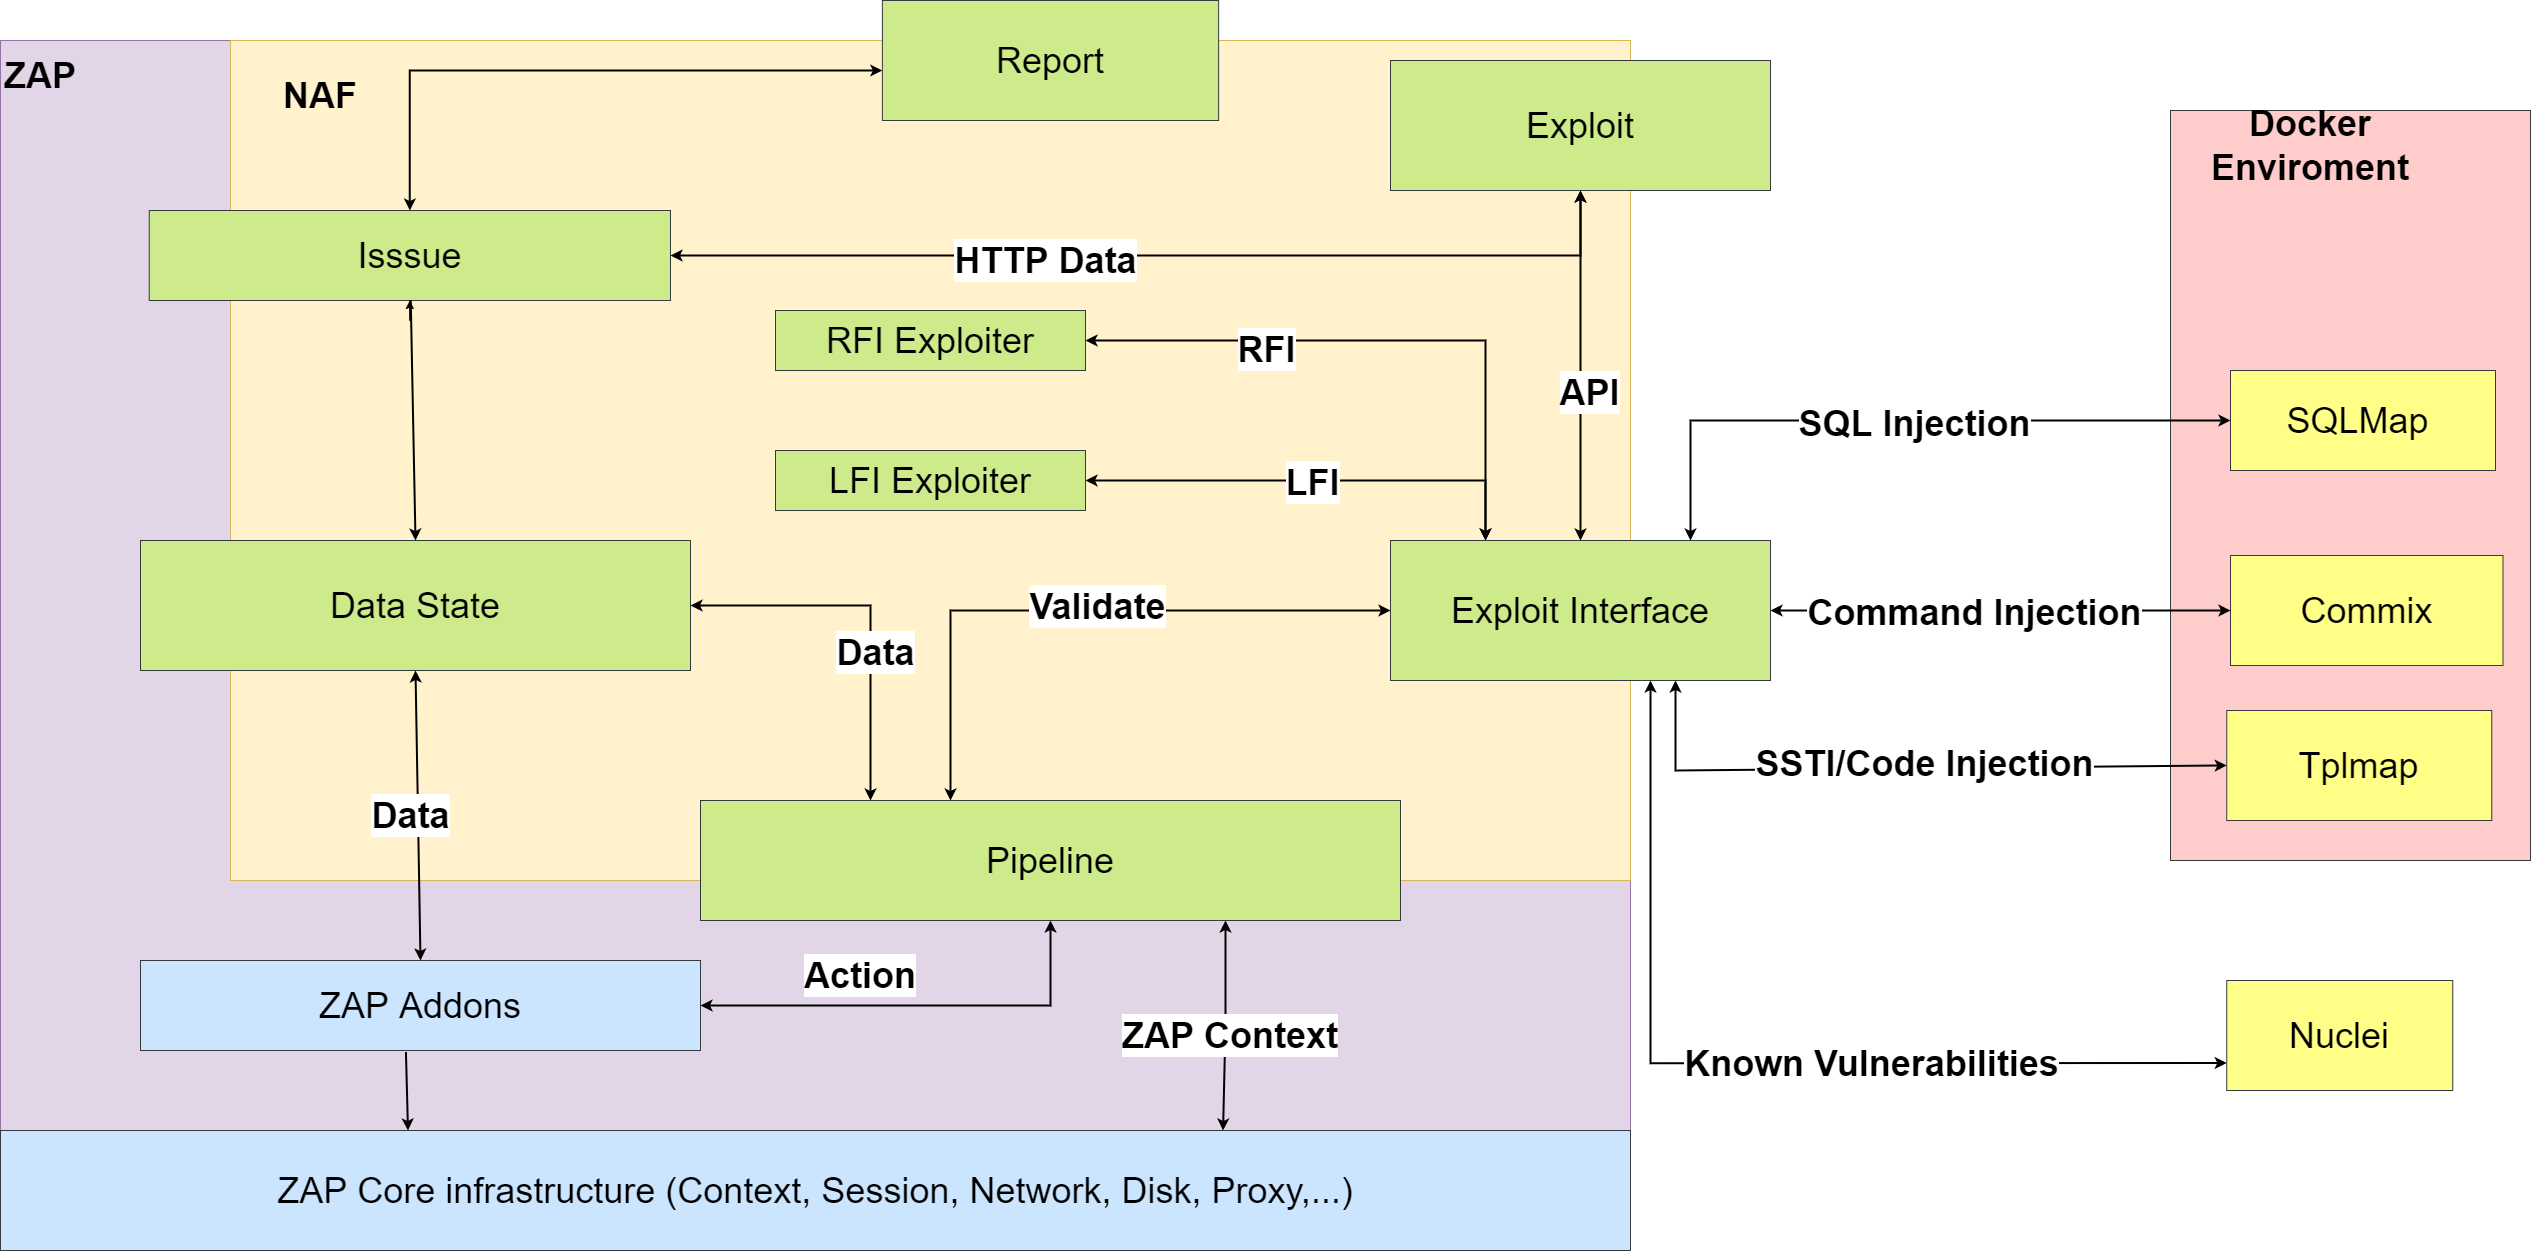
\includegraphics[width=\linewidth]{./images/component.png}
	\caption{Biểu đồ phụ thuộc của các Component}
	\label{fig:component}
\end{figure}

Đối với ngôn ngữ triển khai em lựa chọn, Kotlin là một ngôn ngữ JVM có thể tương tác được với Java để phát triển.

\begin{figure}[H]
	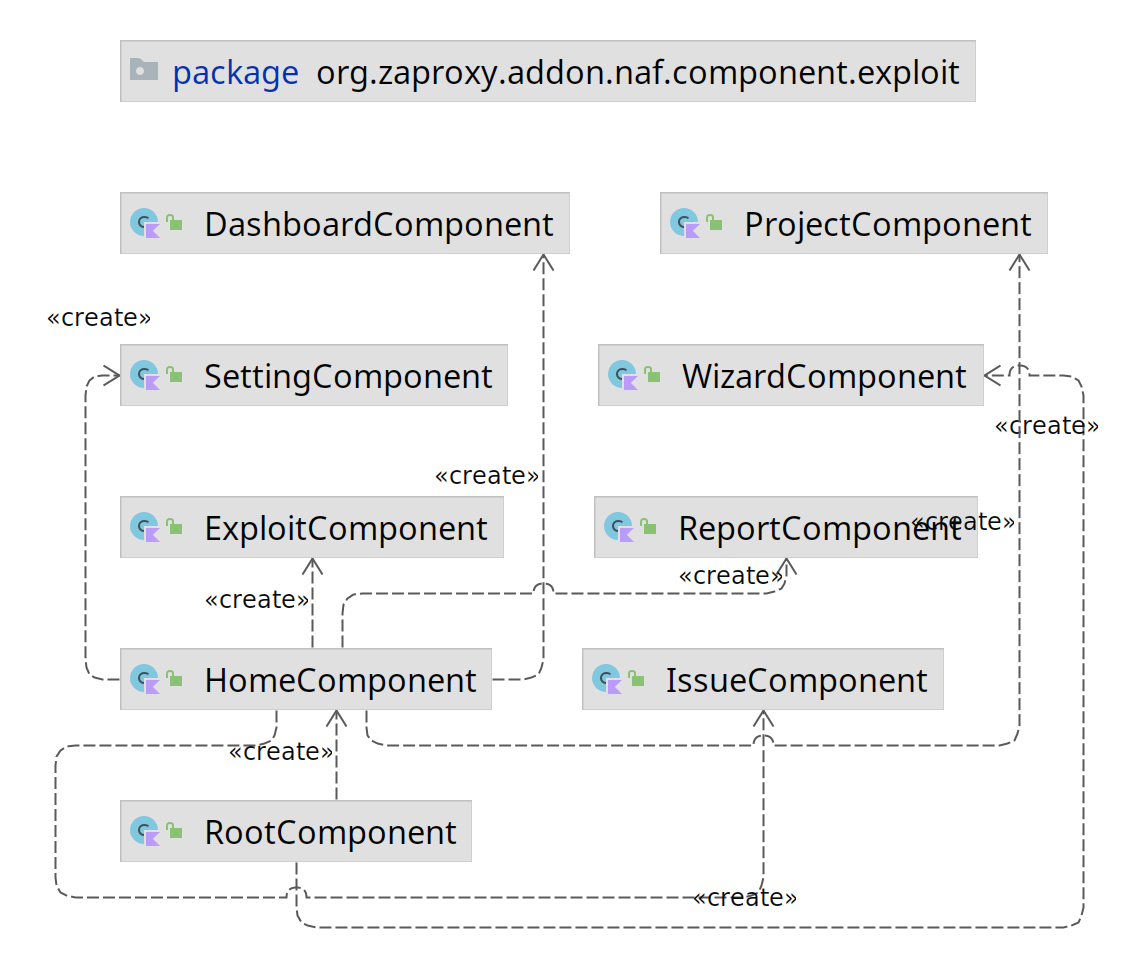
\includegraphics[width=\linewidth]{./images/package.png}
	\caption{Tổ chức component trong mã nguồn}
	\label{fig:package}
\end{figure}

Về triển khai UI và tổ chức mã nguồn, em lựa chọn Jetpack Compose và Decompose làm các thư viện chính để phát triển UI và tổ chức Component thay cho Swing - một thư viện khá cũ và khó tổ chức khi đưa cả Logic và UI vào chung một mã nguồn.

\subsection{Kiến trúc kiểm thử tự động theo Pipeline}
Như đã nêu vấn đề ở trên, ZAP sử dụng các Addons như một phần nên việc thích hợp các công cụ xác minh tự động khá khó. Do đó, em xây dựng một đường ống (Pipeline) để tương tác được với ZAP Core, sử dụng được với các ZAP Addons khác, đồng thời có thể thêm các chi tiết khác vào quá trình kiểm thử tự động.

Mỗi đoạn ống sẽ thuộc về các pha của kiểm thử, pha có độ ưu tiên cao được thực hiện trước để cung cấp thông tin cho các pha sau.

Các pha bao gồm: Khởi tạo, Fuzz, Crawl, Rà quét.

Kiến trúc có thể biểu diễn dưới dạng các thành phần sau
\begin{itemize}
	\item Ngữ cảnh quét là thành phần chứa thông tin của các cuộc tìm kiếm lỗ hổng tự động, các đoạn của đường ống sẽ sử dụng thông tin này để thực hiện các hoạt động của mình một cách động lập trên toàn đường ống. Ngữ cảnh quét ánh xạ tới các thành phần ZAP Core.
	\item Đường ống là quá trình liên tục chứa các đoạn, tại đây diễn ra việc tìm lỗ hổng tự động và xác minh tự động.
	\item Các đoạn của đường ống là các đơn vị chạy các việc để thực hiện quá trình kiểm thử tự động.
\end{itemize}

\subsubsection{Khởi tạo}

Đối với các đoạn của đường ống như khởi tạo ngữ cảnh thì cần có tương tác trực tiếp với cả ZAP Core và cả đường ống.

Các tương tác này được xử lý như sau
\begin{itemize}
	\item Thiết lập ngữ cảnh riêng cho việc kiểm thử: Mỗi lần kiểm thử tự động nên có một ngữ cảnh riêng ứng với đó là một ngữ cảnh của ZAP riêng chứa các thông tin về thông tin cho việc sử dụng Proxy, Crawler, Scanner,...
	\item Thiết lập mục tiêu (Target) cho kiểm thử: Thực hiện truy cập vào truy vấn tới URL mục tiêu, cung cấp cho hệ thống thêm thông tin về Root Site Node, đánh dấu điểm bắt đầu của Sitemap.
	\item Thông tin về các ca kiểm thử được sử dụng. Thông tin được đánh dấu dưới dạng Chính sách (Policy)
	      \begin{itemize}
		      \item Về công nghệ sử dụng: Được cung cấp qua tập công nghệ sử dụng (Tech Set) trong ZAP Context, Scanner sẽ sử dụng thông tin này để lựa chọn phù hợp để kiểm thử, đối với trường hợp thông thường tập công nghệ được đánh dấu toàn bộ sẽ khiến lượng ca kiểm thử trở lên rất lớn.
		      \item Về ngưỡng cảnh báo: Các ca kiểm thử đều có ngưỡng cảnh báo riêng dựa trên hành vi của hệ thống đối với ca kiểm thử, mức độ càng thấp tăng lượng âm tính giả càng lớn ngược lại làm tăng mức dương tính giả.
		      \item Mức độ cảnh báo: Thiết lập để phù hợp với các mục tiêu kiểm thử, mức độ này sẽ được trả về hệ thống thông qua cơ chế Thông báo (Alert)
	      \end{itemize}
	      \begin{figure}[H]
		      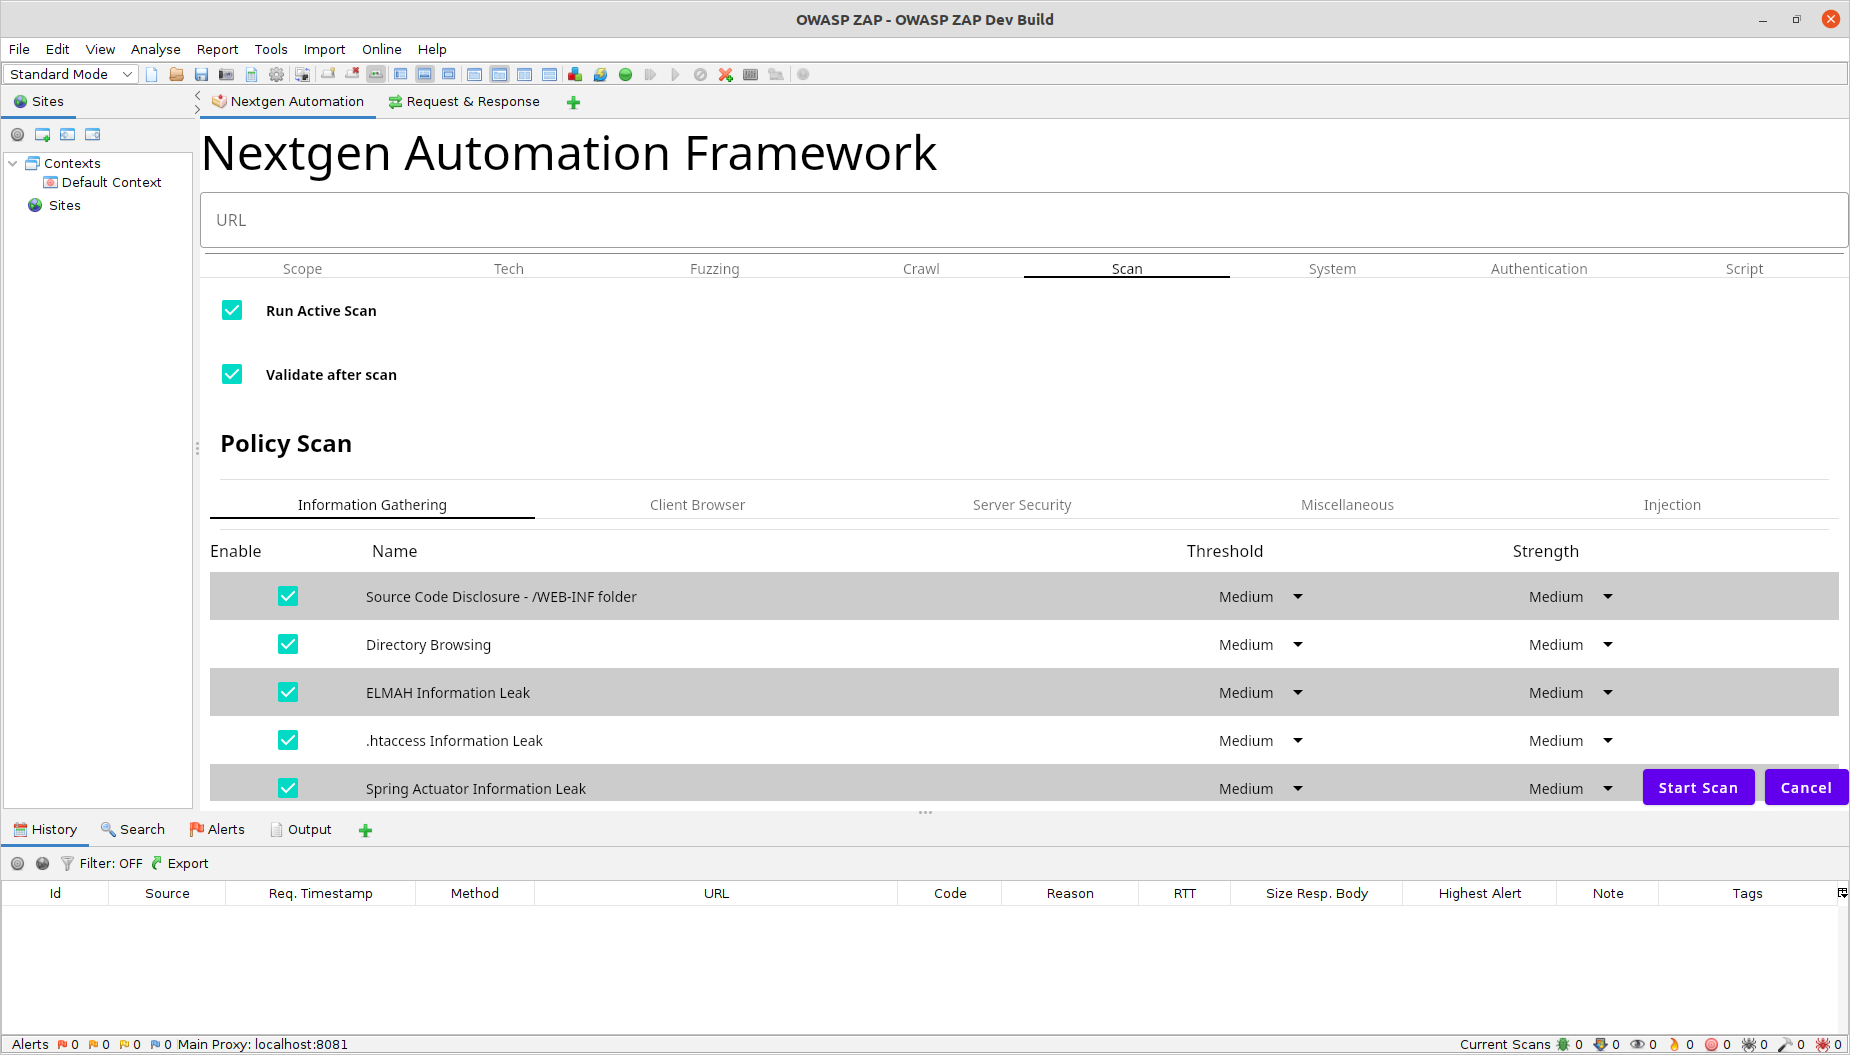
\includegraphics[width=\linewidth]{./images/policy.png}
		      \caption{ Điều chỉnh các các chính sách }
		      \label{fig:policy}
	      \end{figure}
	\item Thông tin về xác thực: Cần được thực hiện một lần đăng nhập “ảo” để lấy thông tin để cung cấp đầy đủ thông tin cho ZAP Context. ZAP Context sẽ “hướng dẫn” Crawler, Scanner thực hiện đăng nhập khi bị đăng xuất. Các thông tin cần được cung cấp bao gồm:
	      \begin{itemize}
		      \item Trang đăng nhập
		      \item Thông tin về yêu cầu đăng nhập
		      \item Thông tin ủy nhiệm (Credential)
		      \item Biểu hiện khi đã đăng nhập/đăng xuất.
	      \end{itemize}
	      \begin{figure}[H]
		      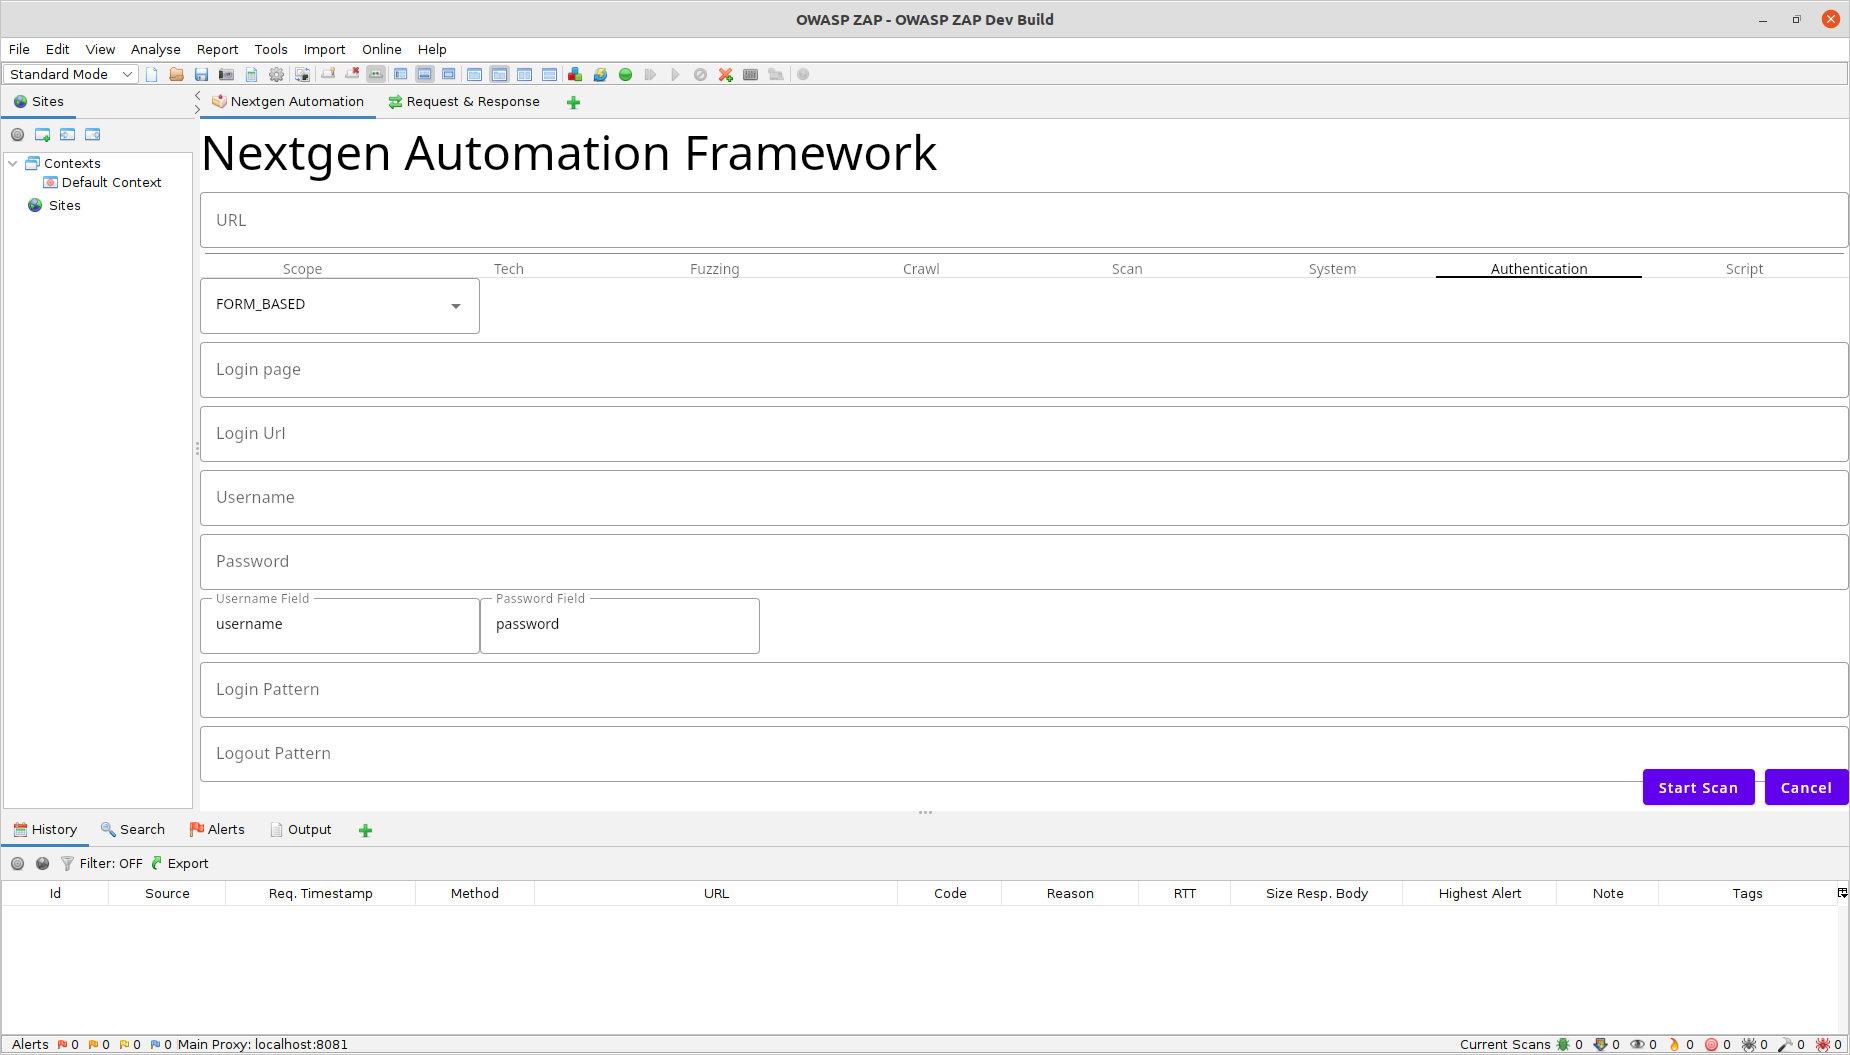
\includegraphics[width=\linewidth]{./images/authen.png}
		      \caption{ Đưa ra thông tin xác thực }
		      \label{fig:authen}
	      \end{figure}

\end{itemize}
Với các thông tin trên nên được thực hiện tự động và ẩn đi phần logic phức tạp trên, người dùng chỉ nên được tương tác thông qua một trình Wizard.

Các thông tin này được em triển khai bằng cách giữ lại nhưng một trạng thái có thể lưu lại, chỉ được thực hiện khi bắt đầu quá trình kiểm thử tự động. Khi kiểm thử tự động sẽ dựa vào các thông tin này để sinh ra các thiết lập để đưa vào ZAP Core một cách tự động.

\subsubsection{Fuzzing Url}
Một việc cần thiết là để ZAP có thể hoạt động hiệu quả cung cấp thêm thông tin về cấu trúc của Website cho ZAP. Một trong những phương pháp phổ biến cho việc này là vét cạn các điểm cuối thường có của một Website theo từ điển (thường được sử dụng với tên Fuzzing). Kỹ thuật này hiệu quả với việc kiểm thử hộp đen và hộp xám khi không có hoặc có rất ít các thông tin về hệ thống. Ngoài ra, nó cũng giúp phát hiện ra có lỗ hổng do việc thiết lập cấu hình không an toàn.

Cộng đồng phát triển ZAP đã phát triển một Addons là Forced Browsing trên cơ sở sử dụng thư viện DirBuster có hiệu quả khá cao trong việc Fuzzing cũng như cung cấp một vài Wordlist phổ biến cho việc Fuzzing. Pipeline này sẽ sử dụng hai Addons trên và Wordlist được cung cấp (người dùng lựa chọn) để thực hiện việc Fuzzing này. Việc này cũng được thiết đặt tự động trong trình Wizard thay vì phải thiết lập thủ công.

Đây là một trong Element đầu tiên trong Pipeline, Addons Forced Browsing tương đối hoàn thiện, chỉ cần dựa trên Wordlist được người dùng lựa chọn và các tùy chọn để thực hiện Fuzzing và cố gắng thu thập lại lượng endpoint phù hợp để sinh ra lượng Site Node lớn nhất để có thông tin về Website.

\begin{figure}[H]
	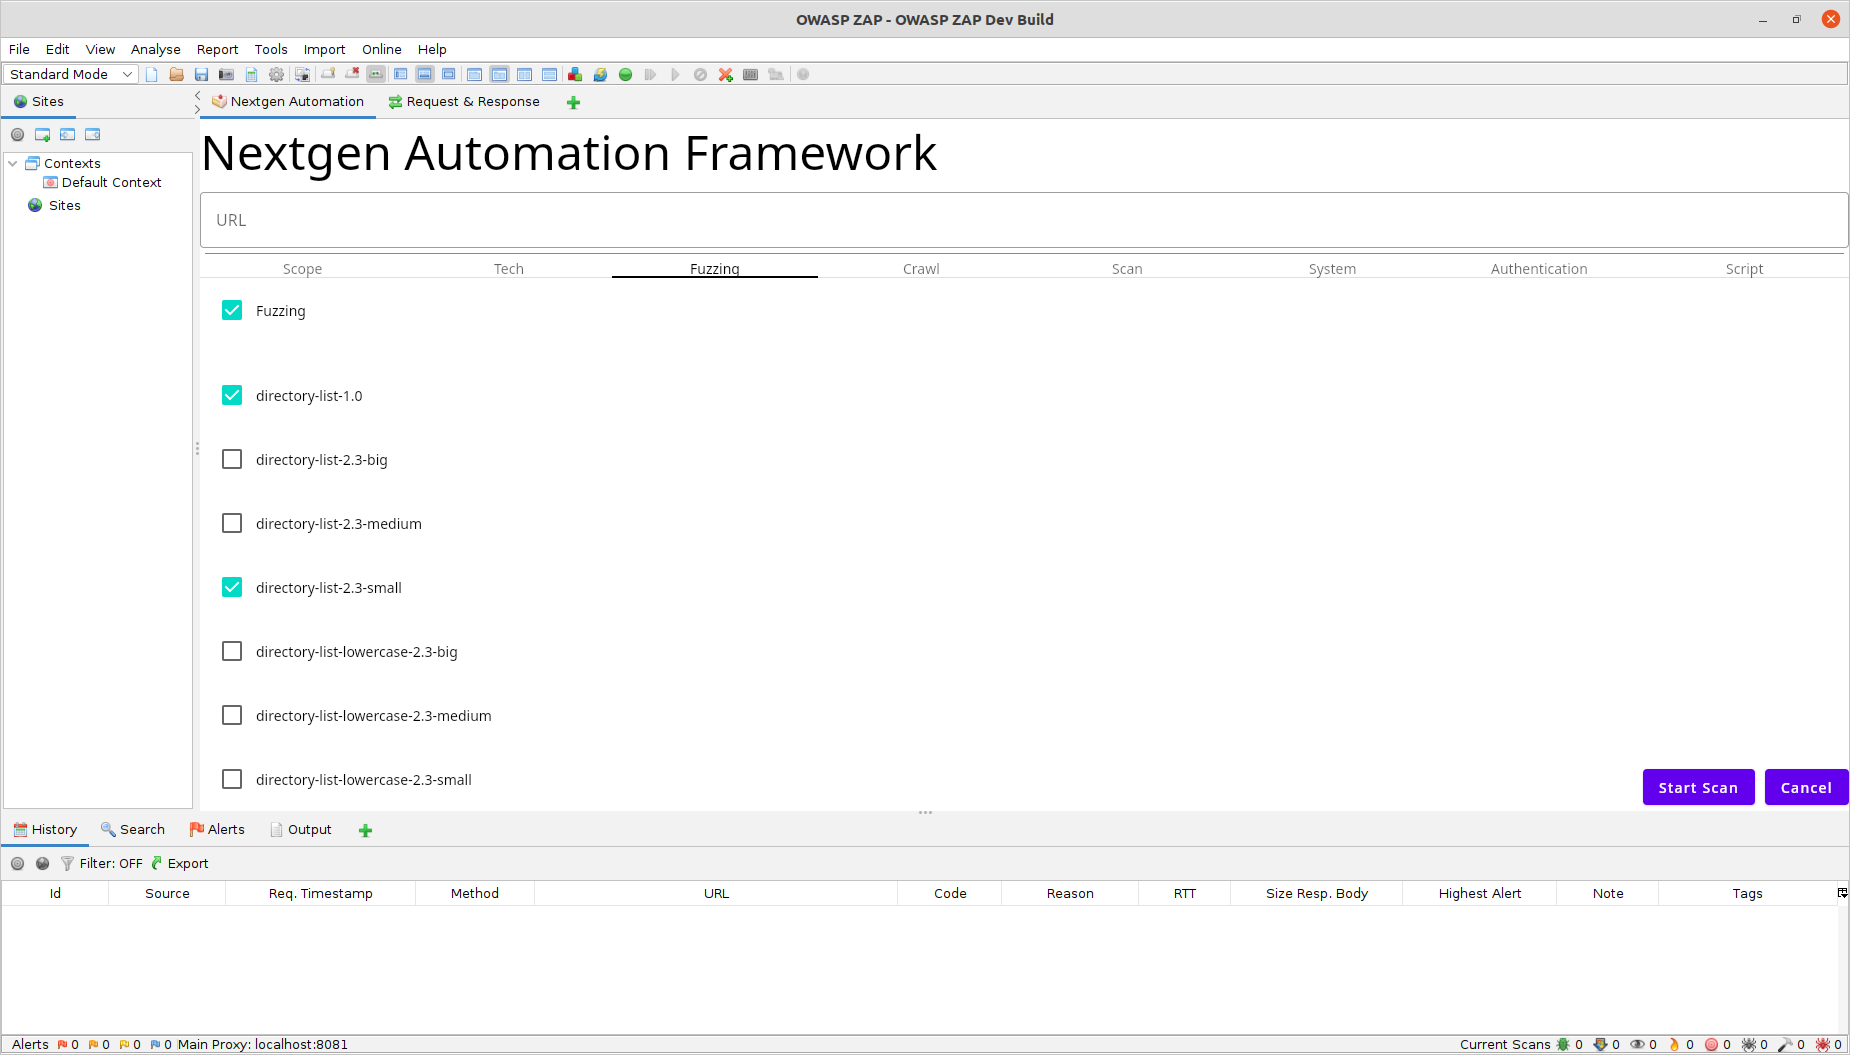
\includegraphics[width=\linewidth]{./images/fuzz.png}
	\caption{Tùy chọn Wordlist để Fuzzing}
	\label{fig:fuzz}
\end{figure}

\subsubsection{Crawl}

Một cách nữa để cung cấp thông tin về cấu trúc của Website là cào (Crawl) dữ liệu trên toàn bộ Website để lấy thông tin.

Đội ngũ phát triển ZAP cũng đã phát triển hai Addons là Spider và Ajax Spider. Spider được sử dụng để cào dữ liệu, thông tin lấy từ cây DOM của Website trong các phản hồi của các yêu cầu HTTP.

Đối với một số Website sẽ sử dụng thêm Ajax để lấy thông tin từ máy chủ, các Crawler tĩnh như Spider sẽ không phát hiện được các yêu cầu này. Đội ngũ phát triển ZAP cũng đã phát triển thêm Ajax Spider, công cụ xây dựng dựa trên Selenium để thực hiện việc cào dữ liệu trực tiếp bằng Selenium đấy được thông tin về các yêu cầu thực hiện thông qua Ajax bằng cách thực thi Javascript như một trình duyệt thực.

Hai Addons được phát triển và duy trì liên tục nên có hiệu quả rất cao trong việc thực hiện cào dữ liệu. Do là một trong các Addons Core nên hai Addons này cần sử dụng trực tiếp các thông tin từ ngữ cảnh của ZAP Core. Để tự động được các Addons này cần đồng thời xử lý thông tin ở ZAP Context trước khi gửi thông tin cho Addons và thực thiện gọi các Addons thực hiện theo trình tự của của các pha.

các Pipeline Element này có mục tiêu là tối ưu hóa việc cào dữ liệu từ DOM và các yêu cầu Ajax. Để cho crawler hoạt động tốt nhất cần cung cấp ZAP Context chứa các thông tin về phạm vi và thông tin đăng nhập để quá trình Crawl không bị hủy bỏ do vấn đề xác thực.
\subsubsection{Scan}

Đây là pha chính trong việc kiểm thử an ninh, tại đây các luật (Rule) của cộng đồng đóng góp sẽ được sử dụng để kiểm tra các hành vi của hệ thống để suy diễn ra các lỗ hổng của hệ thống. Cộng đồng phát triển ZAP đã phát triển hai Addons là Passive Scan và Active Scan. Tuy nhiên, Passive Scan lại chỉ phù hợp khi thực hiện kiểm thử thủ công hoặc bán tự động. Active Scan là công cụ hiệu quả cho việc chạy các luật được đưa ra của Policy trong ngữ cảnh của ZAP. Chính công cụ này sẽ đóng thực hiện việc thử các luật, loại bỏ bớt các luật dựa trên Tech Set được đưa vào, lựa chọn các ca kiểm thử phù hợp với độ nhạy và đưa ra cảnh báo dựa trên mức độ cảnh bảo.

Pipeline Element hoạt động dựa trên Policy đã được cung cấp để đưa ra cảnh báo. Quá trình này cũng cần được cung cấp ZAP Context để có thể thực hiện ca kiểm thử mà không hủy bỏ do vấn đề xác thực. Đồng thời cũng nên đưa vào các vùng nguy hiểm trong Scope để tránh làm lỗ hệ thống (ví dụ các thiết lập tài khoản, hệ thống).

Việc cài đặt bước này cần đem được các thông tin từ phase trước kết hợp với thông tin người dùng cung cấp để thực hiện. Các Addons tương đối độc lập nên thông tin đầu ra của từng Addons là khác nhau và không ổn định, các thông tin đầu ra được thu thập, chuẩn hóa và đưa lại vào trong Component trực quan hóa thông tin.

\begin{figure}[H]
	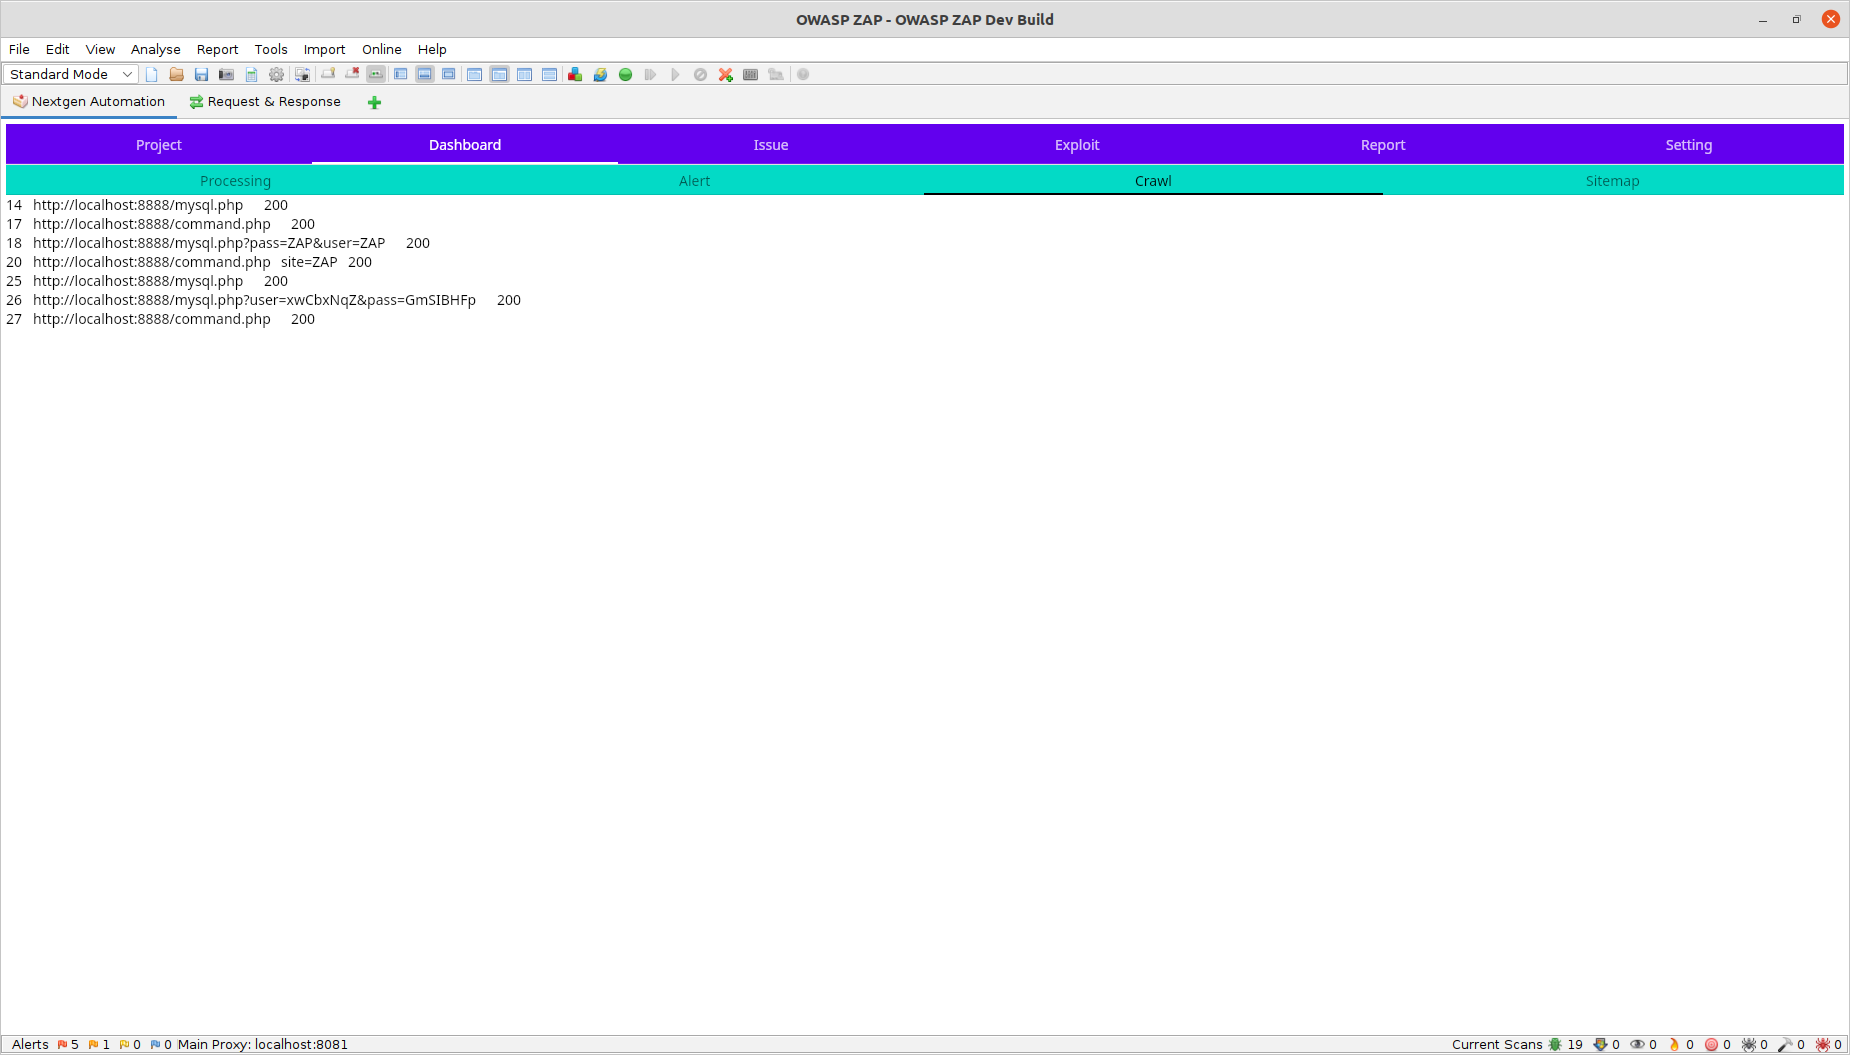
\includegraphics[width=\linewidth]{./images/scan_result.png}
	\caption{Kết quả crawl}
	\label{fig:scan_result}
\end{figure}

\subsection{Thích hợp công cụ xác minh tự động}
Các công cụ xác minh tự động làm nhiệm vụ xác minh lại các cảnh bảo, nếu được xác minh, một Issue mới được tạo ra và được thêm vào cơ sở dữ liệu

Các lỗ hổng cần được xác minh phân chia cho các công cụ như sau
\begin{description}
	\item[SQL Injection] SQLMap
	\item [Command Injection/Code Injection] Commix
	\item [Server Side Template Injection/Code Injection] Tplmap
	\item [Remote File Inclusion] RFIExploiter
	\item [Local File Inclusion/Path Traversal] LFIExploiter
\end{description}
Để xác định được cảnh báo nào thuộc về lỗ hổng nào cần sử dụng đến giá trị định danh của Common Weakness Enumeration (CWE) để xác định tương đối lỗ hổng nào thuộc về loại nào.
\subsubsection{SQLMap}
Công cụ SQLMap, đi kèm với một API Server nên việc giao tiếp có thể thiết lập qua công API Server này. API Server sử dụng là REST-API sử dụng JSON là format để truyền tải thông tin. Tuy nhiên dữ liệu trả về không là có định dạng chuẩn do SQLMap được xây dựng bằng Python là một ngôn ngữ kiểu động. Do đó, cần xây dựng thêm một số Parser riêng để có thế đưa dữ liệu trả về đúng kiểu.

Lúc này các nhiệm vụ khai thác được mô hình hóa thành các Job, API Server sẽ xử lý các Job trong Job Pool và trả về dữ liệu theo các yêu cầu của công cụ gửi lên. Các yêu cầu có thể là xác minh lỗ hổng, lấy các thông tin của cơ sở dữ liệu.


\begin{figure}[H]
	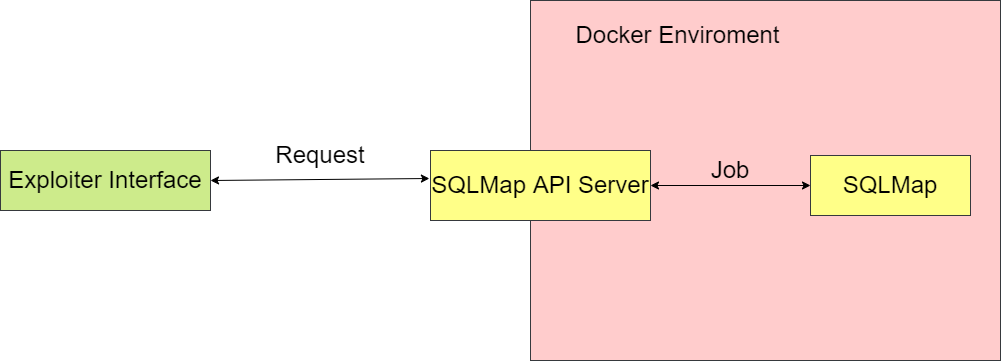
\includegraphics[width=\linewidth]{./images/SQLMap.png}
	\caption{Biểu đồ tương tác giữa SQLMap và công cụ.}
	\label{fig:sqlmap}
\end{figure}

Đối với pha xác minh, SQLMap chỉ cần xác minh là lỗ hổng có tồn tại hay không dựa trên thông tin cảnh báo đưa ra.
\subsubsection{Commix và Tplmpa}
Khác với SQLMap, Commix và Tplmap không có một API Server, các tương tác cần được đưa vào và ra thông qua đầu vào chuẩn (STDIN) và đầu ra chuẩn(STDOUT).

Đối với Docker Engine cũng cần có API giao tiếp gián tiếp để có thể thực thi và lấy được đầu vào chuẩn và đầu ra chuẩn của Container.


\begin{figure}[H]
	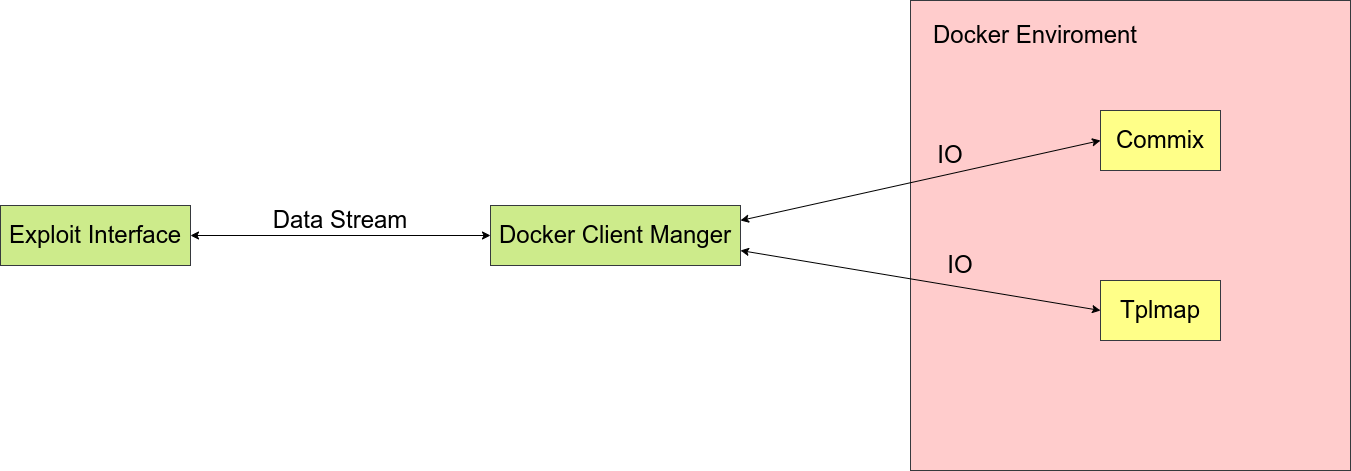
\includegraphics[width=\linewidth]{./images/DockerIO.png}
	\caption{Biểu đồ tương tác công cụ với Commix và Tplmap.}
	\label{fig:commix_tplmap}
\end{figure}

Đối với việc xác minh, Commix và Tplmap sẽ cố gắng thực thi một lệnh và kiểm tra lệnh có được thực thi hay không bằng kiểm tra đầu ra chuẩn để xác minh.

\subsubsection{Remote File Inclusion}
Lỗ hổng này là đặc trưng của PHP nên sẽ chỉ được kiểm tra với PHP. Đưa đường dẫn tới một pha đầu vào chứa một đoạn mã thực thi của PHP, nếu được thực thi thì được xác minh là đúng. Với lỗ hổng này không có các dự án mã nguồn mở để khai thác nên em cần tự triển khai một trình khai thác riêng.
\subsubsection{Local File Inclusion/Path Traversal}
Lỗ hổng này sẽ không cần xác minh lại do độ, nhưng vẫn được xây dựng để phát triển công cụ khai thác. Lỗ hổng này cũng không có dự án mã nguồn mở để khai thác nên em cũng tự triển khai một trình khai thác riêng.

\subsection{Trực quan hóa thông tin}
Dù là các ZAP Addons cung cấp khá đầy đủ các thông tin về thông tin của chính Addons đó cho người dùng nhưng chính sự độc lập của các Addons lại khiến thông tin của toàn bộ ứng dụng ZAP nói chung lại bị phân tán thành tại các vị trí khác nhau. Đồng thời các Addons lại chia sẻ rất ít thông tin cho các Addons khác.

Điều này làm nảy sinh một nhiệm vụ cần được xây dựng là tập hóa các thông tin về quá trình kiểm thử, thông tin thu thập được thành một trang có sức trực quan hóa cao để hiệu quả trong việc theo dõi.

Kiến trúc Event Bus của ZAP Core và các thông tin được cung cấp thêm trực tiếp các Addons khác và các thành phần được thêm vào. Cần thu thập thông tin lượng vừa đủ và chuẩn hóa các thông tin thu thập được thành một miền cố định để có thể trực quan hóa. Như đã nói ở trên, Addons rất ít chia sẻ thông tin ra ngoài nên lượng thông tin em cần thực hiện qua một số kĩ thuật khác với luồng hoạt động thông thường của ZAP để có thể tổng hợp được nhiều và đầy đủ hơn lượng thông tin.

\begin{figure}[H]
	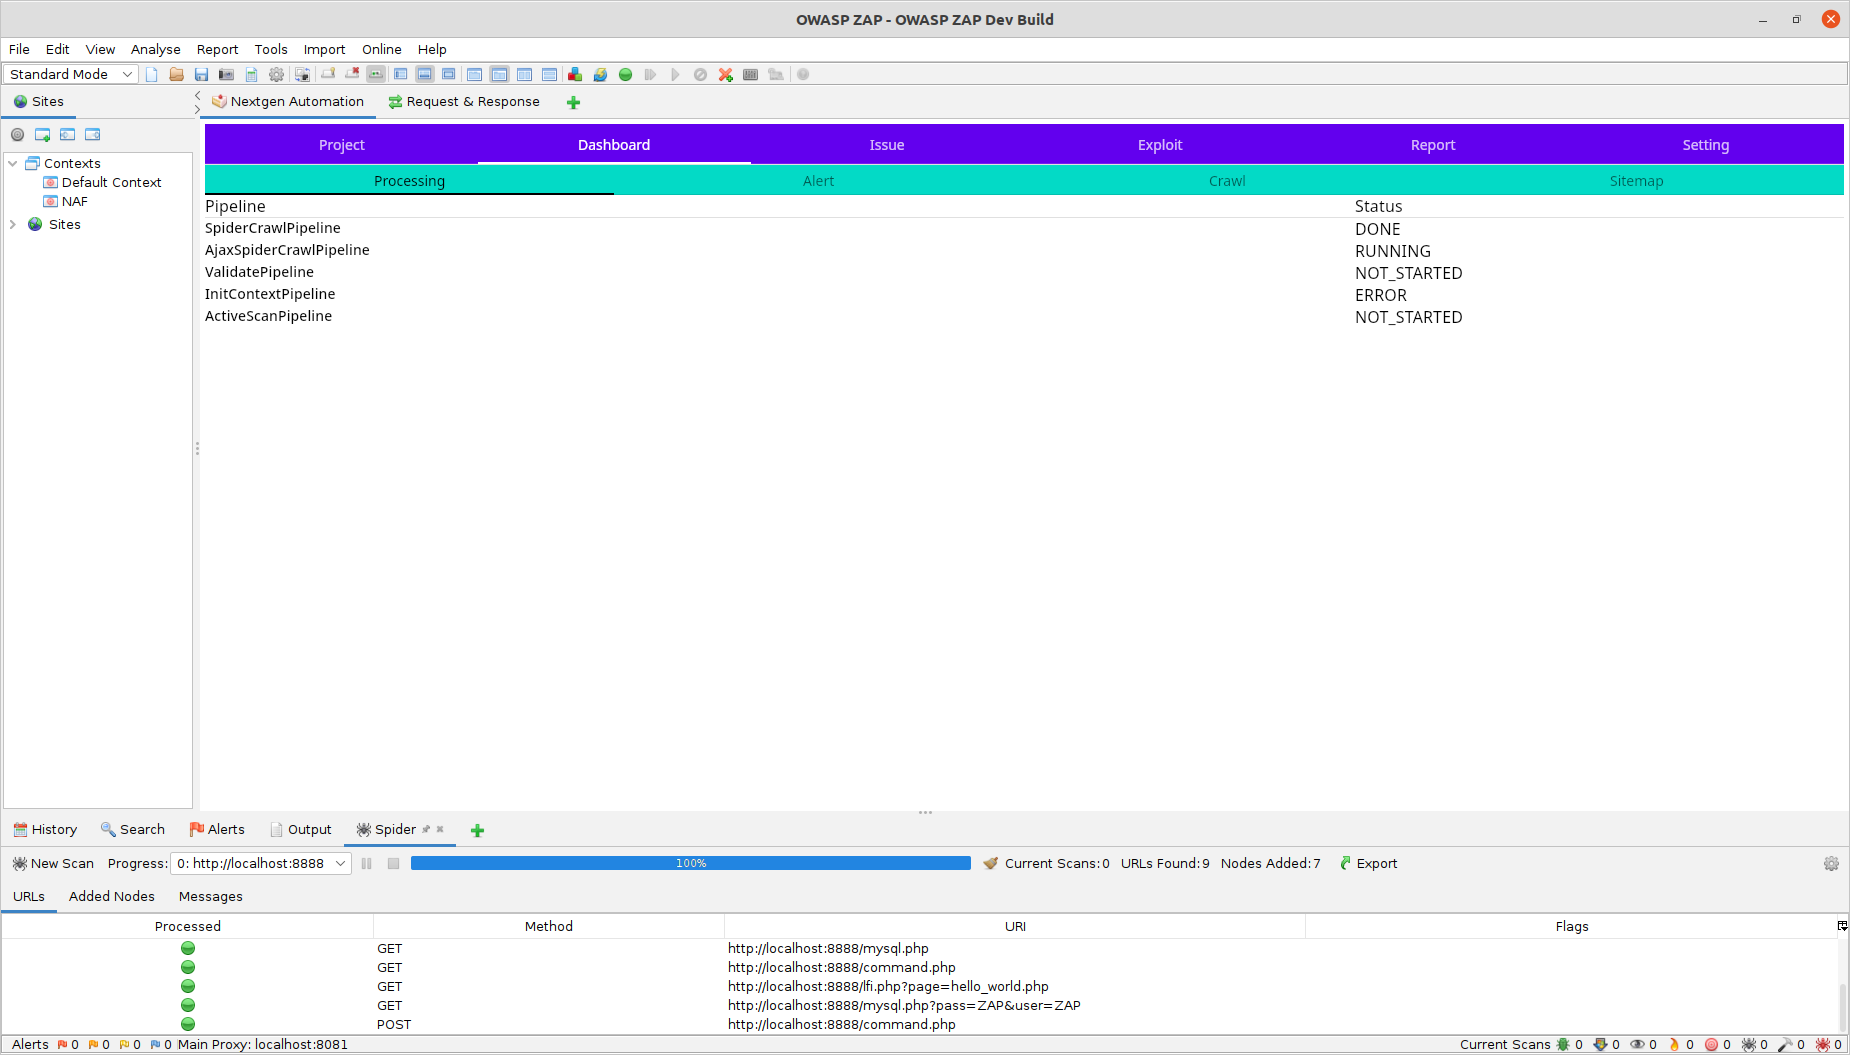
\includegraphics[width=\linewidth]{./images/state.png}
	\caption{Thanh trạng thái pipeline đang chạy}
	\label{fig:state}
\end{figure}

\subsection{Quản lý Issue và sinh báo cáo}
Theo luồng được cộng đồng ZAP định ra, thì cảnh bảo (Alert) là đơn vị được sử dụng để quản lý các lỗ hổng được sinh ra từ ZAP, tuy nhiên điều này hơi không phù hợp do hai lý do. Một là lượng cảnh báo mà ZAP sinh ra rất lớn và được sinh ra liên tục dẫn đến cần được xác thực lại liên tục. Hai là mục tiêu cuối cùng là cần sinh ra được báo cáo bao gồm thông tin chi tiết, cách tái hiện và gợi ý về cách xử lý cho phía phát triển xử lý. Điều này dẫn để cần chuẩn hóa lại các miền để phù hợp với mục đích cuối cùng là giúp nhà phát triển và vấn hành xử lý được các lỗ hổng tồn tại.

Từ đó em đã mô hình hóa lại thành Issue để xử lý hai vấn đề ở trên: chỉ sử dụng cảnh báo nhưng một nguồn và định thông tin tiêu chuẩn để báo cáo xử lý và cho phép xuất ra một bản báo cáo dạng rich text để cung cấp đủ thông tin về lỗ hổng.

Các cảnh báo có thể gửi tới các tab khai thác.

\begin{figure}[H]
	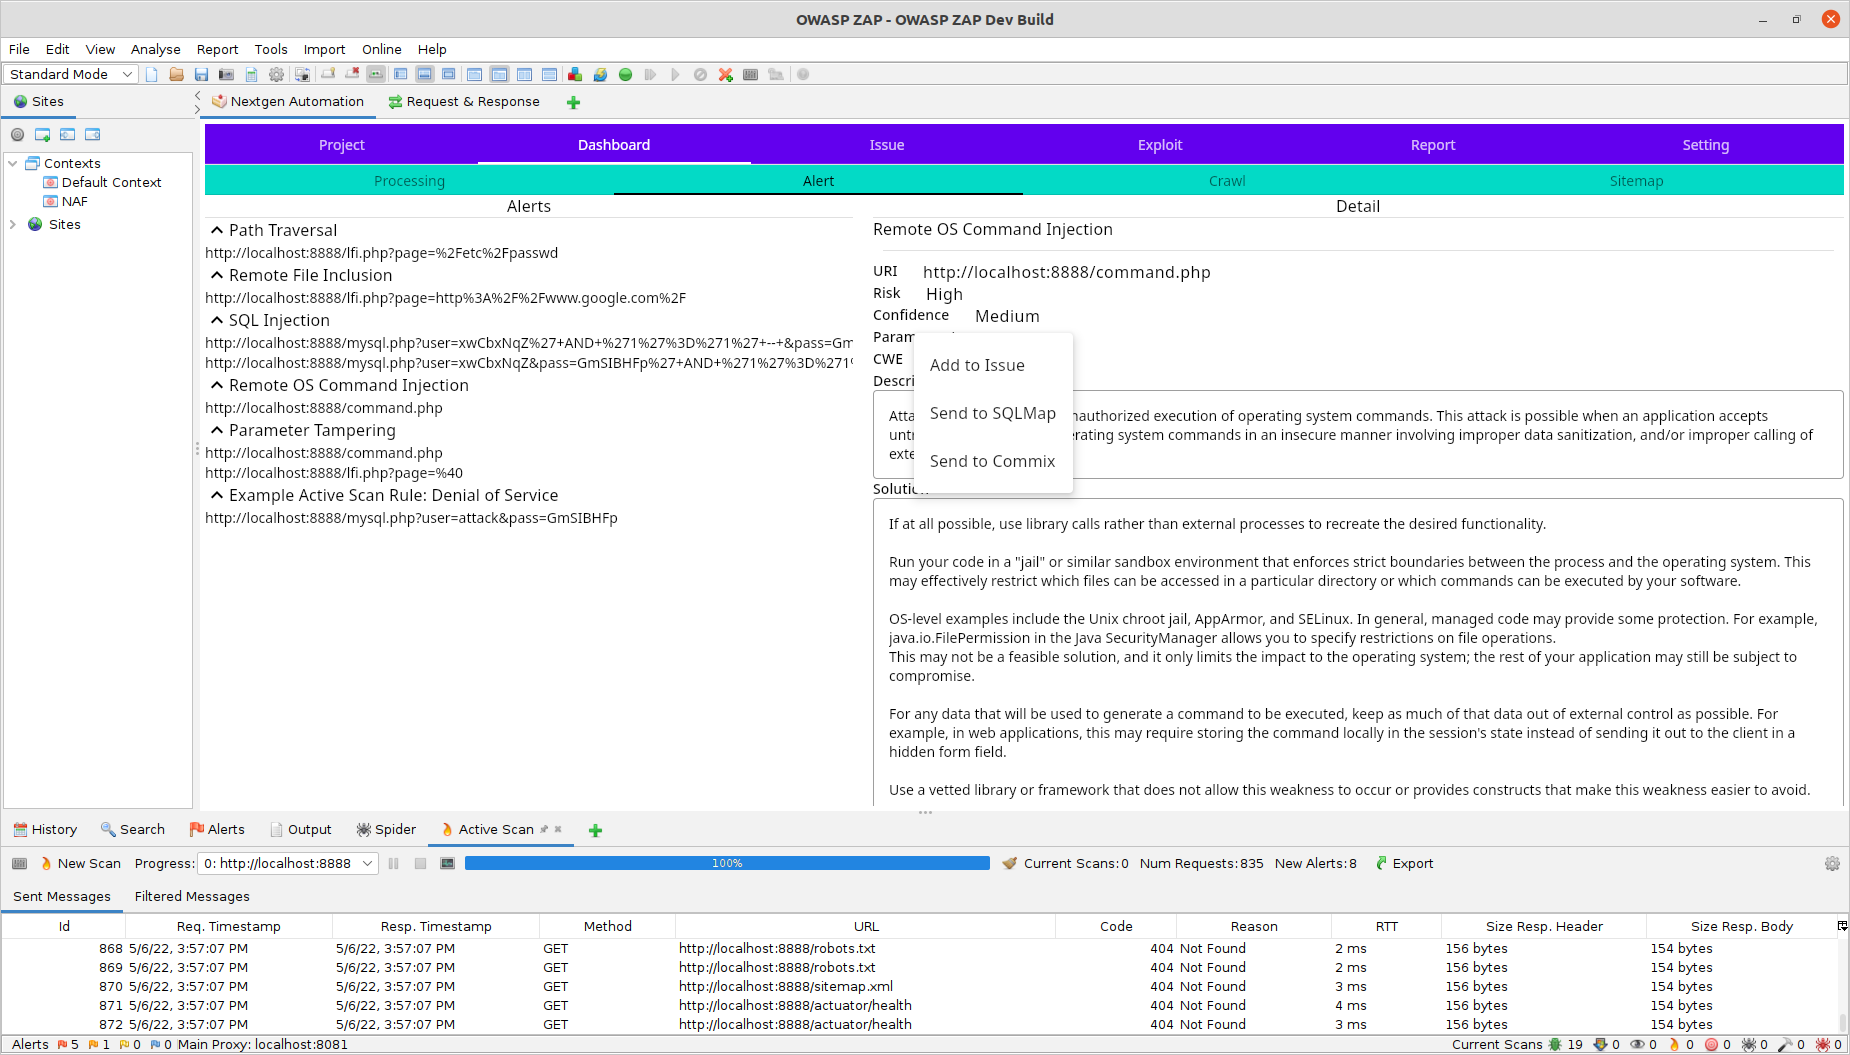
\includegraphics[width=\linewidth]{./images/alert.png}
	\caption{Quản lý alert chung của các công cụ thích hợp}
	\label{fig:alert}
\end{figure}

Báo cáo sinh ra cho phép sử dụng Issue không phải trạng thái UNKNOWN để tạo ra một File PDF chứa báo cáo với format định trước.

\begin{figure}[H]
	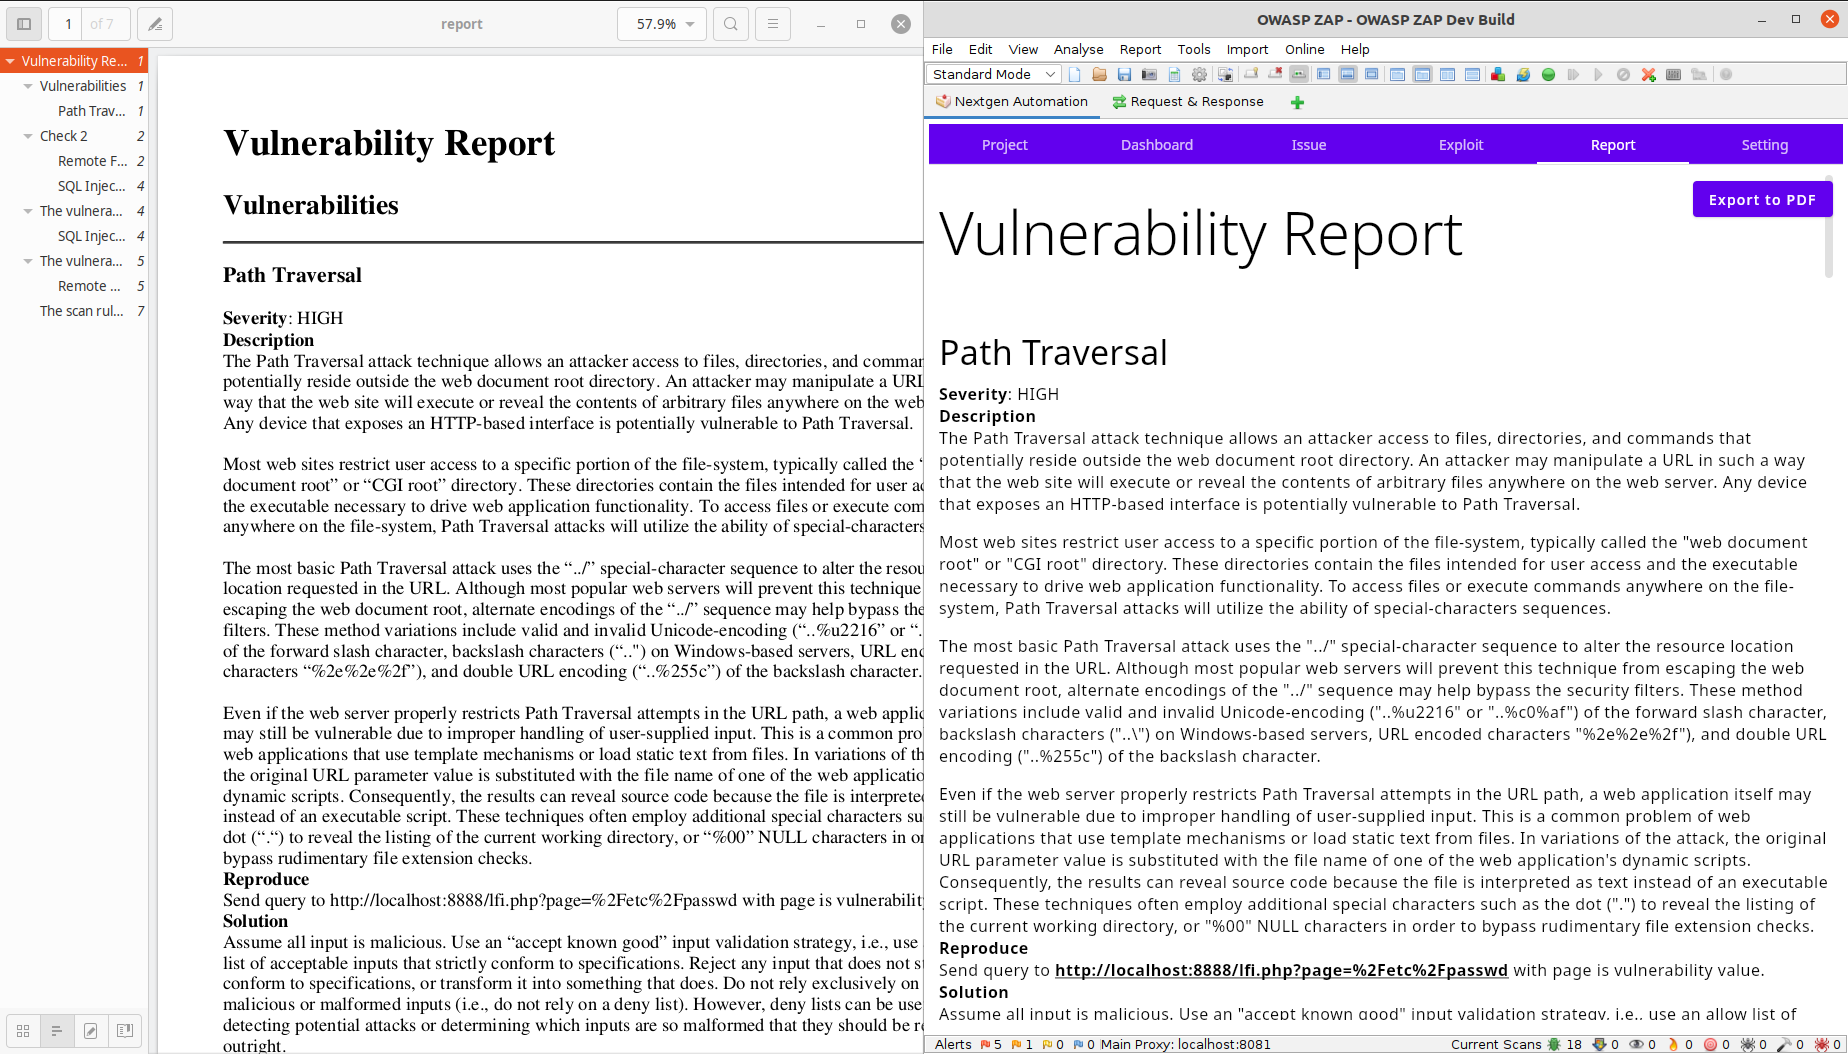
\includegraphics[width=\linewidth]{./images/report.png}
	\caption{Sinh báo cáo cho các lỗ hổng.}
	\label{fig:report}
\end{figure}

\subsection{Các công cụ khai thác và hậu khai thác}

Ngoài việc xác minh tự động trong đường ống, các công cụ thích hợp còn có thể sử dụng như một công cụ khai thác tự động trong ZAP. Việc thích hợp sử dụng chung các thành phần chính với công cụ xác minh tự động.

Để thuận tiện cho việc khai thác thì có thể tạo ra nhiều nhãn (Tab) khai thác khác nhau, mỗi nhãn này là các yêu cầu khai thác khác nhau. Tuy nhiên, đặc điểm chung là các nhãn này sẽ không bao giờ được lưu lại khi hết phiên để tránh lộ thông tin do các vấn đề về an toàn.
\subsubsection{SQLMap}
Với lỗ hổng này, người dùng có thể khai thác từ một cách tự động bằng cách trích xuất các thông tin từ lỗ hổng.

\begin{figure}[H]
	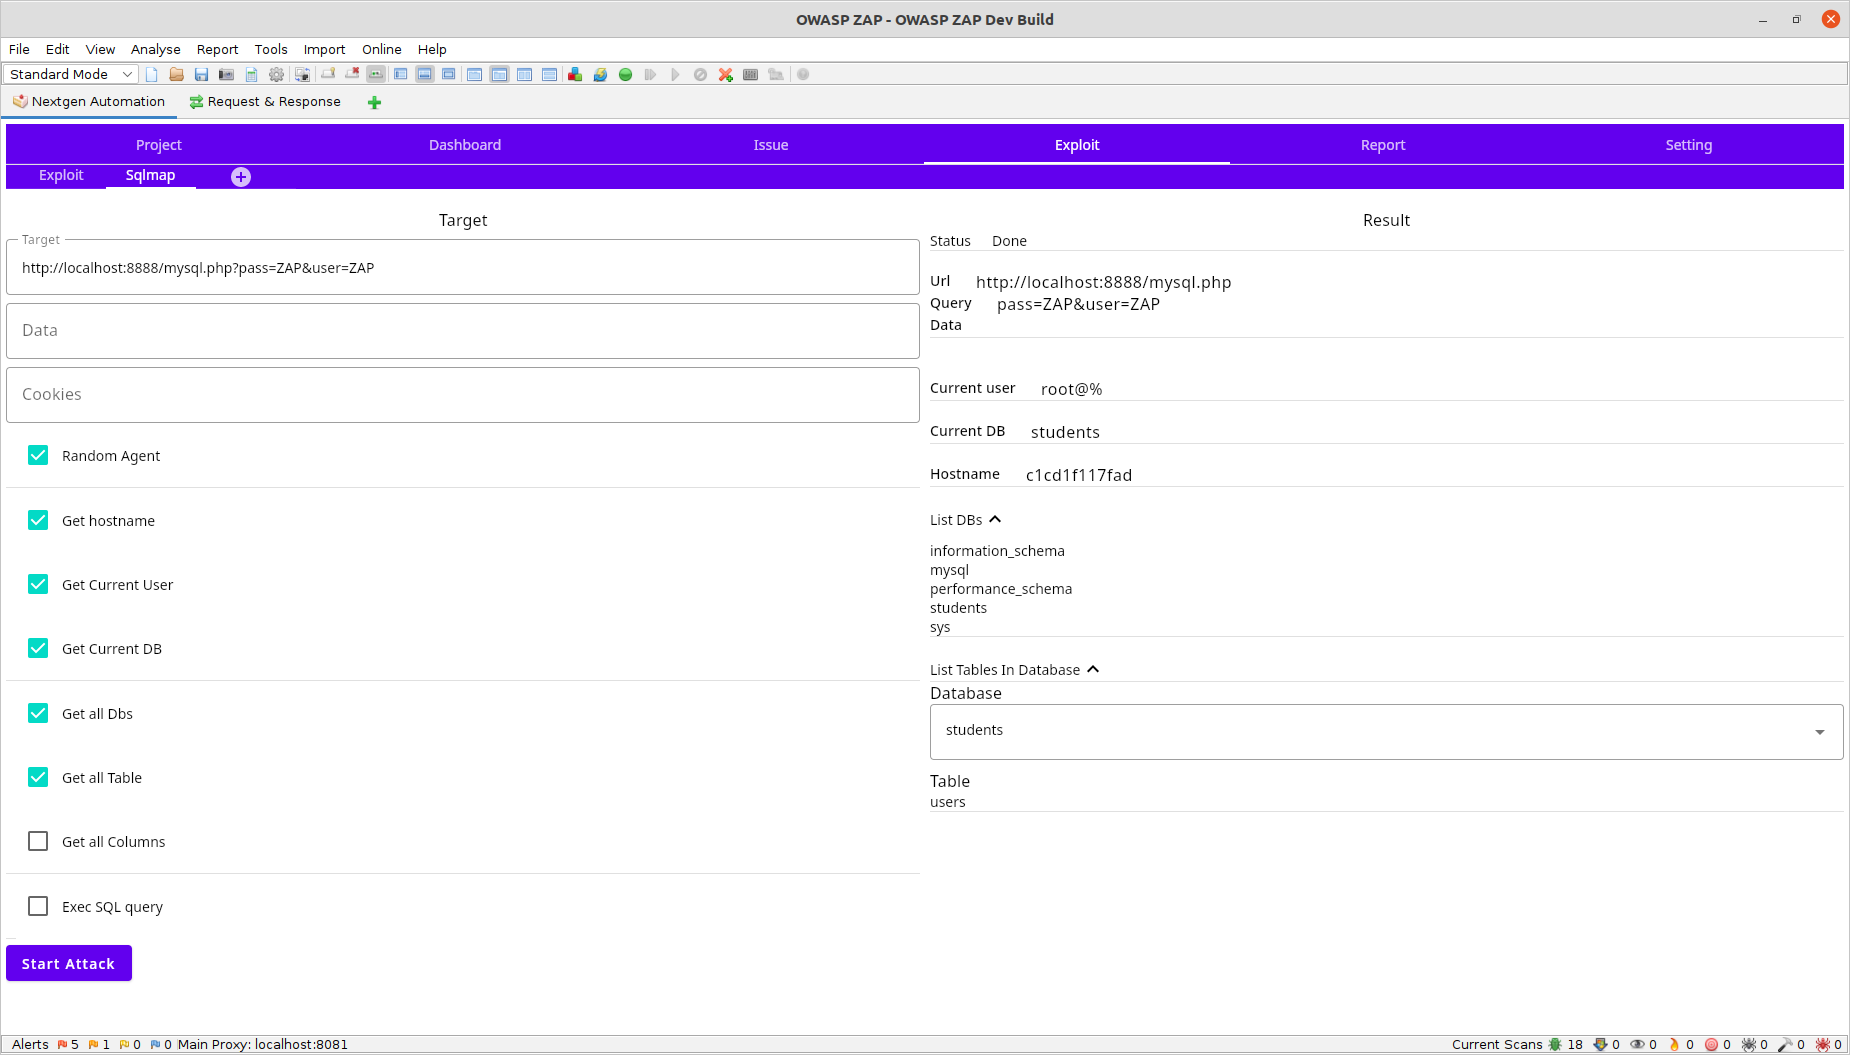
\includegraphics[width=\linewidth]{./images/sqlmap_explot.png}
	\caption{Khai thác lỗ hổng SQL Injection thông qua SQLMap}
	\label{fig:sqlmap_explot}
\end{figure}
Dữ liệu đầu vào có thể gửi trực tiếp từ các cảnh báo tới, các dữ liệu như URL, Cookie, Data sẽ được gửi cùng sang để việc khai thác trở nên ngắn gọn hơn hoặc tự chỉnh sửa để dễ dàng xác nhận hơn.
\subsubsection{Commix}

Dữ liệu đầu vào cũng có thể gửi từ cảnh báo sang tương tự SQLMap.

\begin{figure}[H]
	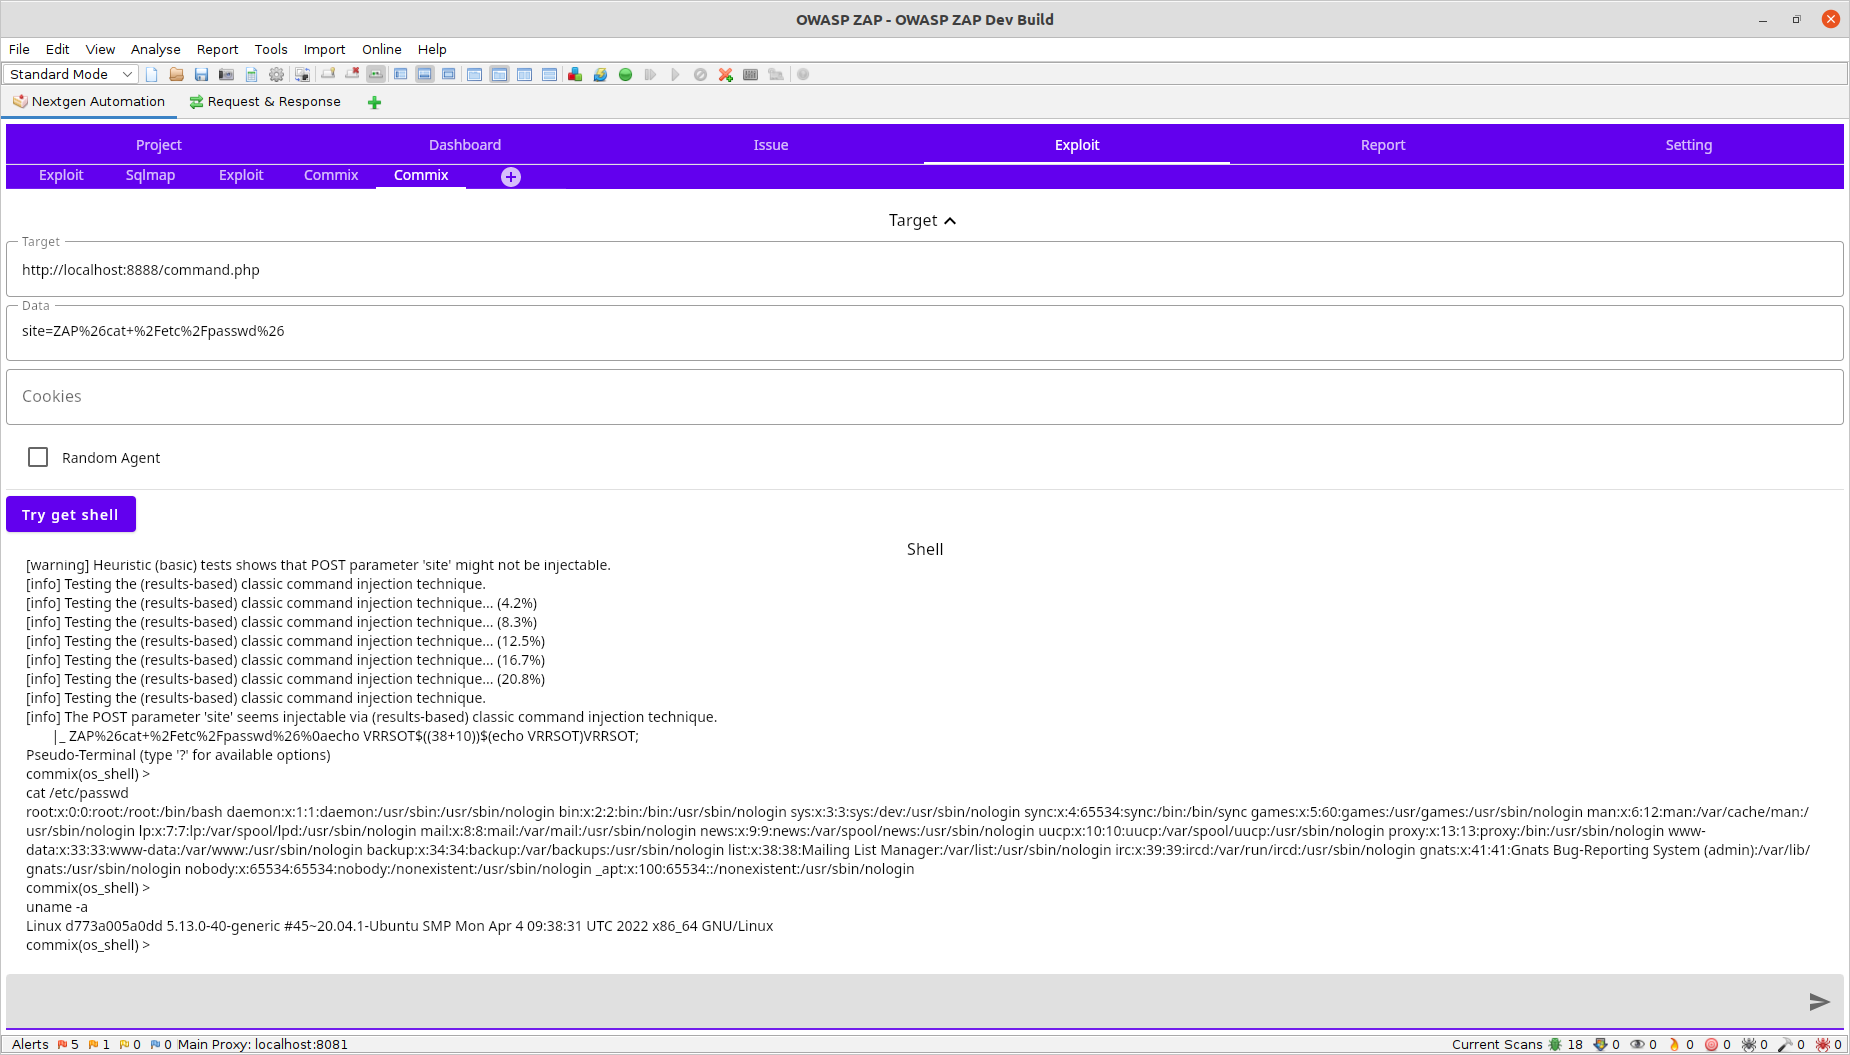
\includegraphics[width=\linewidth]{./images/commix_exploit.png}
	\caption{Khai thác lỗ hổng OS Command Injection bằng Commix	}
	\label{fig:commix_exploit}
\end{figure}
Các câu lệnh sẽ được gửi tới Commix và nhận về output tương tự một trình pseudo-shell.
\subsubsection{Tplmap}
Tương tự SQLMap và Commix, Tplmap  câu lệnh khởi tạo có thể được gửi sang từ một cảnh báo.

\begin{figure}[H]
	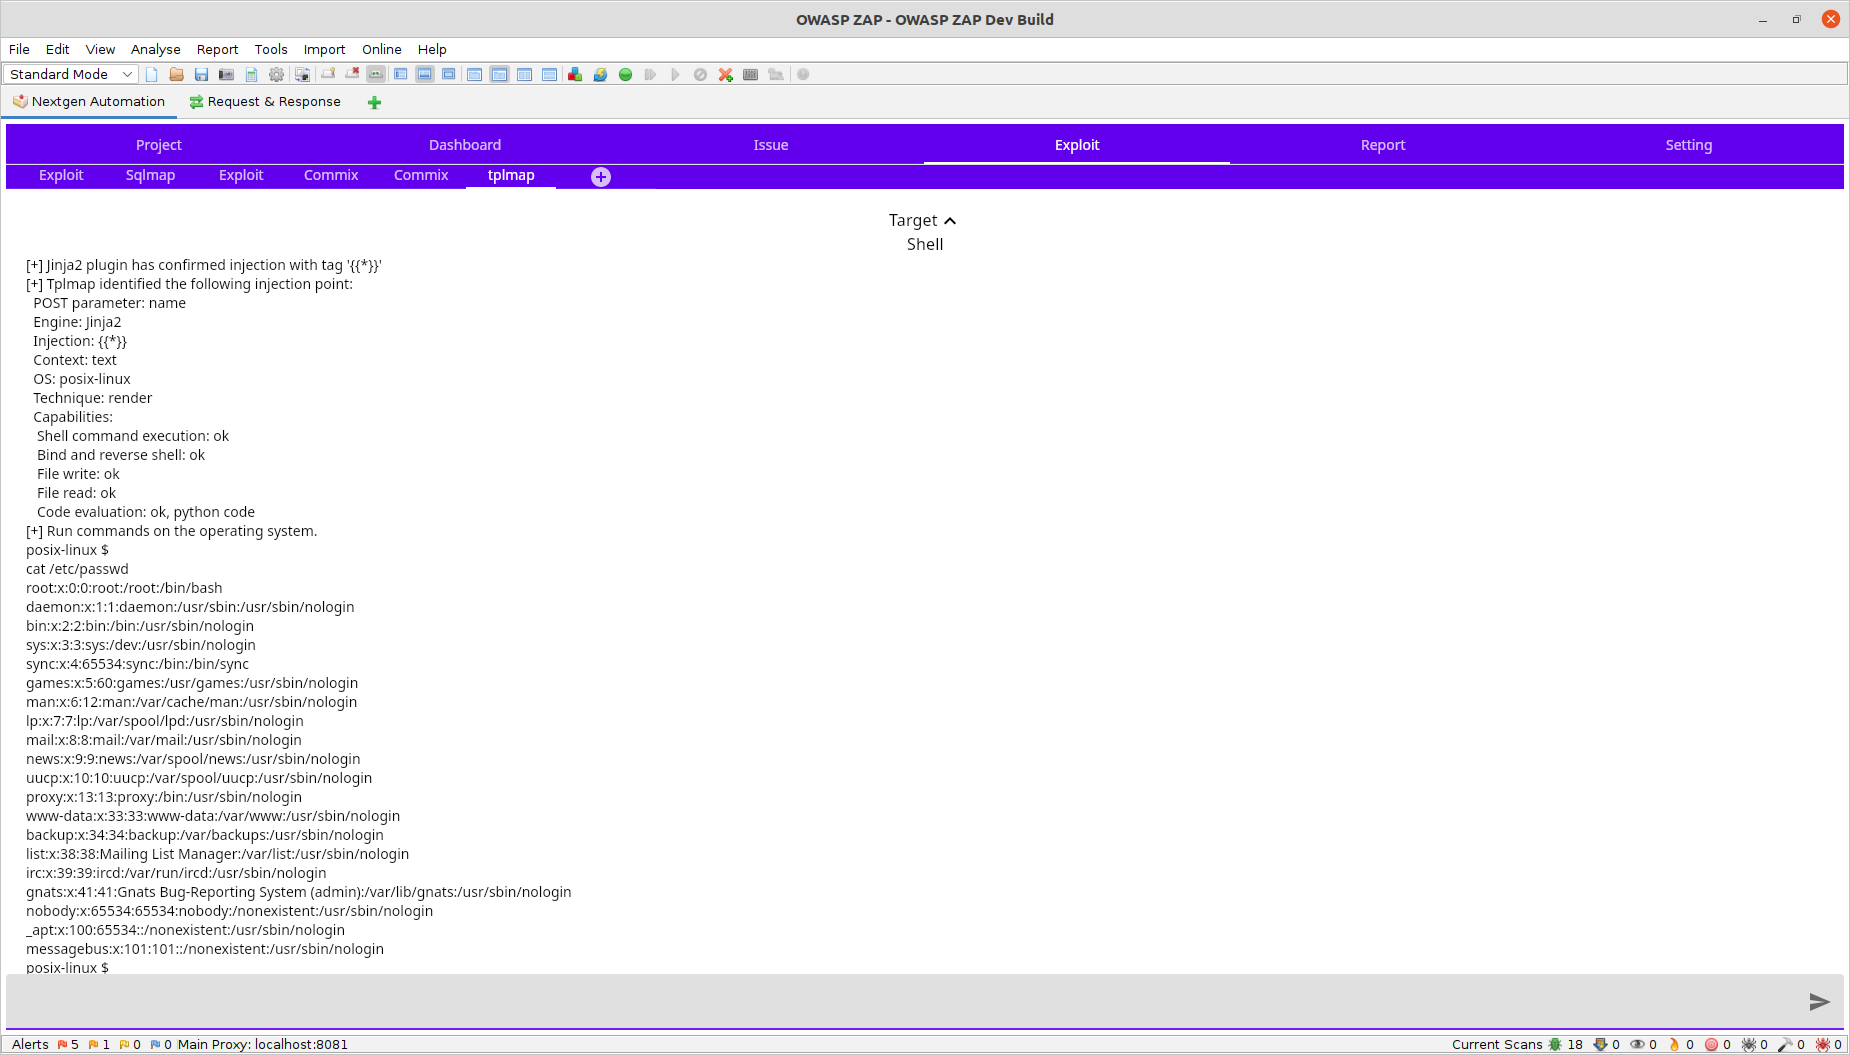
\includegraphics[width=\linewidth]{./images/tplmap_exploit.png}
	\caption{Khai thác lỗ hổng SSTI bằng Tplmap}
	\label{fig:tplmap_exploit}
\end{figure}
Các câu lệnh trong Tplmap cũng được cài đặt để nhận một đầu vào và một đầu ra nhưng một trình pseudo-shell.

\subsubsection{Remote File Inclusion}

Việc khai thác Remote File Inclusion PHP được em triển khai bằng cách thông qua một tập tin thực thi tự triển khai được công khai trên Internet. Trong đây sẽ có một số tham số cho phép mình thực thi lệnh, các đầu ra của lệnh sẽ được gửi về bằng cách phân tích phản hồi của yêu cầu.

\begin{figure}[H]
	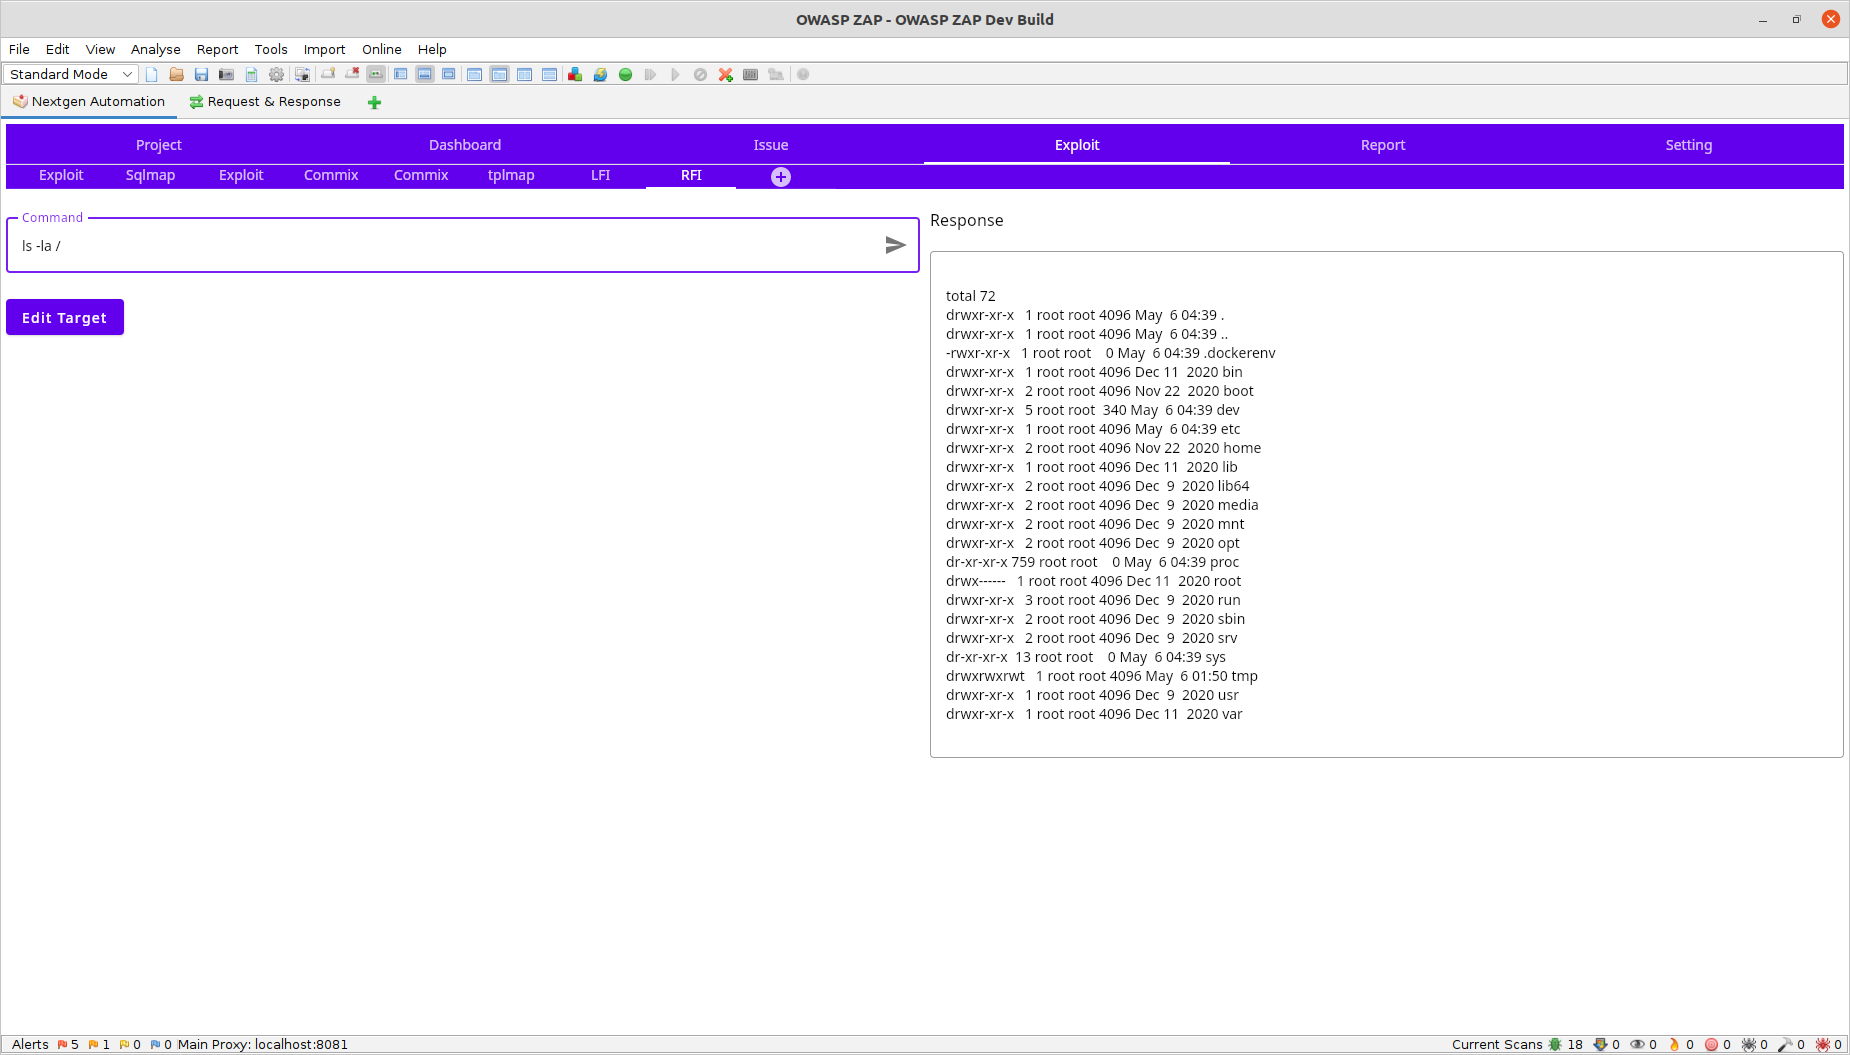
\includegraphics[width=\linewidth]{./images/rfi_exploit.png}
	\caption{Khai thác lỗ hổng RFI bằng RFI Exploiter}
	\label{fig:rfi_exploit}
\end{figure}
\subsubsection{Local File Inclusion/Path Traversal}

Trình khai thác lỗ hổng Local File Inclusion/Path Traversal được em triển khai bằng cách cho phép người dùng lựa chọn một số đường dẫn và thay đổi các đường dẫn để lấy dữ liệu về, người dùng có thể xem dữ liệu trả về thông qua việc quan sát phản hồi.

\begin{figure}[H]
	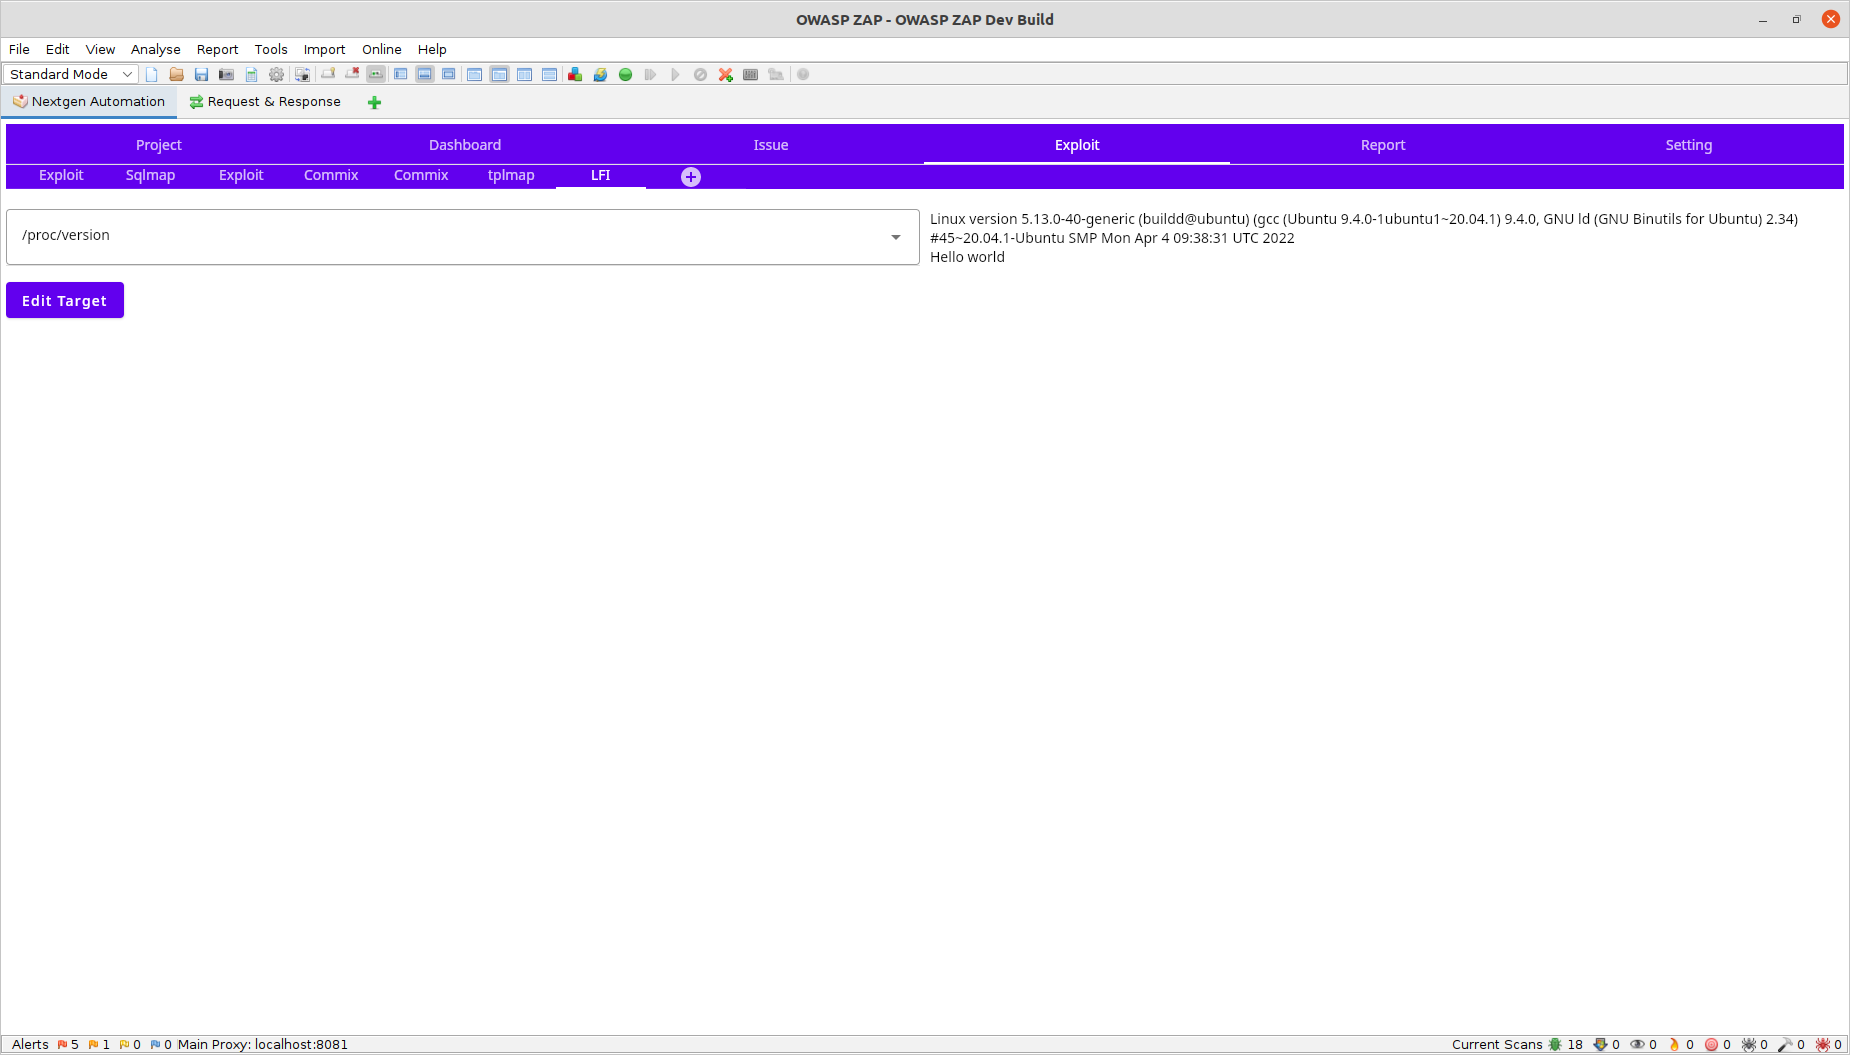
\includegraphics[width=\linewidth]{./images/lfi_exploit.png}
	\caption{Khai thác LFI/Path Traversal bằng công cụ LFI Exploiter}
	\label{fig:lfi_exploit}
\end{figure}
\subsection{Đóng gói các thành phần}

Ngoài việc cần có các Interface để giao tiếp với từng công cụ mã nguồn mở khác nhau thì cũng cần đóng gói các công cụ mở rộng vào thành một Addons hoàn chỉnh. Để giảm thiểu các cài đặt thêm để chạy được các công cụ mở rộng thì em lựa chọn Docker để đóng gói.

Điều này có lợi ích sẽ giúp các công cụ được đóng gói toàn diện, chạy được đa nền tảng tương tự ZAP. Docker cũng là một nền tảng ảo hóa được sử dụng ngày càng phổ biến nên cho phép công cụ dễ dàng thích nghi hơn.

Sự lựa chọn tối ưu để đóng gói các thành phần mà vẫn đem lại hiệu xuất tốt cho các công cụ mở rộng là sử dụng Docker.

Docker có cung cấp Interface để giao tiếp với Docker Daemon thông qua REST-API. Java và Kotlin không được hỗ trợ chính thức các thư viện để giao tiếp nhưng cộng đồng có các thư viện để giao tiếp tuy nhiên đã cũ và có rất ít tài liệu hướng dẫn nên cần bọc lại cung cấp một API hoàn chỉnh hơn cho các Component sử dụng.

Các API này bao gồm
\begin{itemize}
	\item Việc xây dựng các Docker Image chứa các công cụ ở ngoài.
	\item Tạo Container để phù hợp với các tác vụ.
	\item Giao tiếp với các Container.
	\item Xóa bỏ các Container không sử dụng.
\end{itemize}

Để sử dụng các Container hiệu quả, các các Container nên được đặt có các Network Interface cùng với hệ điều hành để tránh việc kết nối bị từ chối do Container sử dụng một mạng ảo riêng.

\begin{figure}[H]
	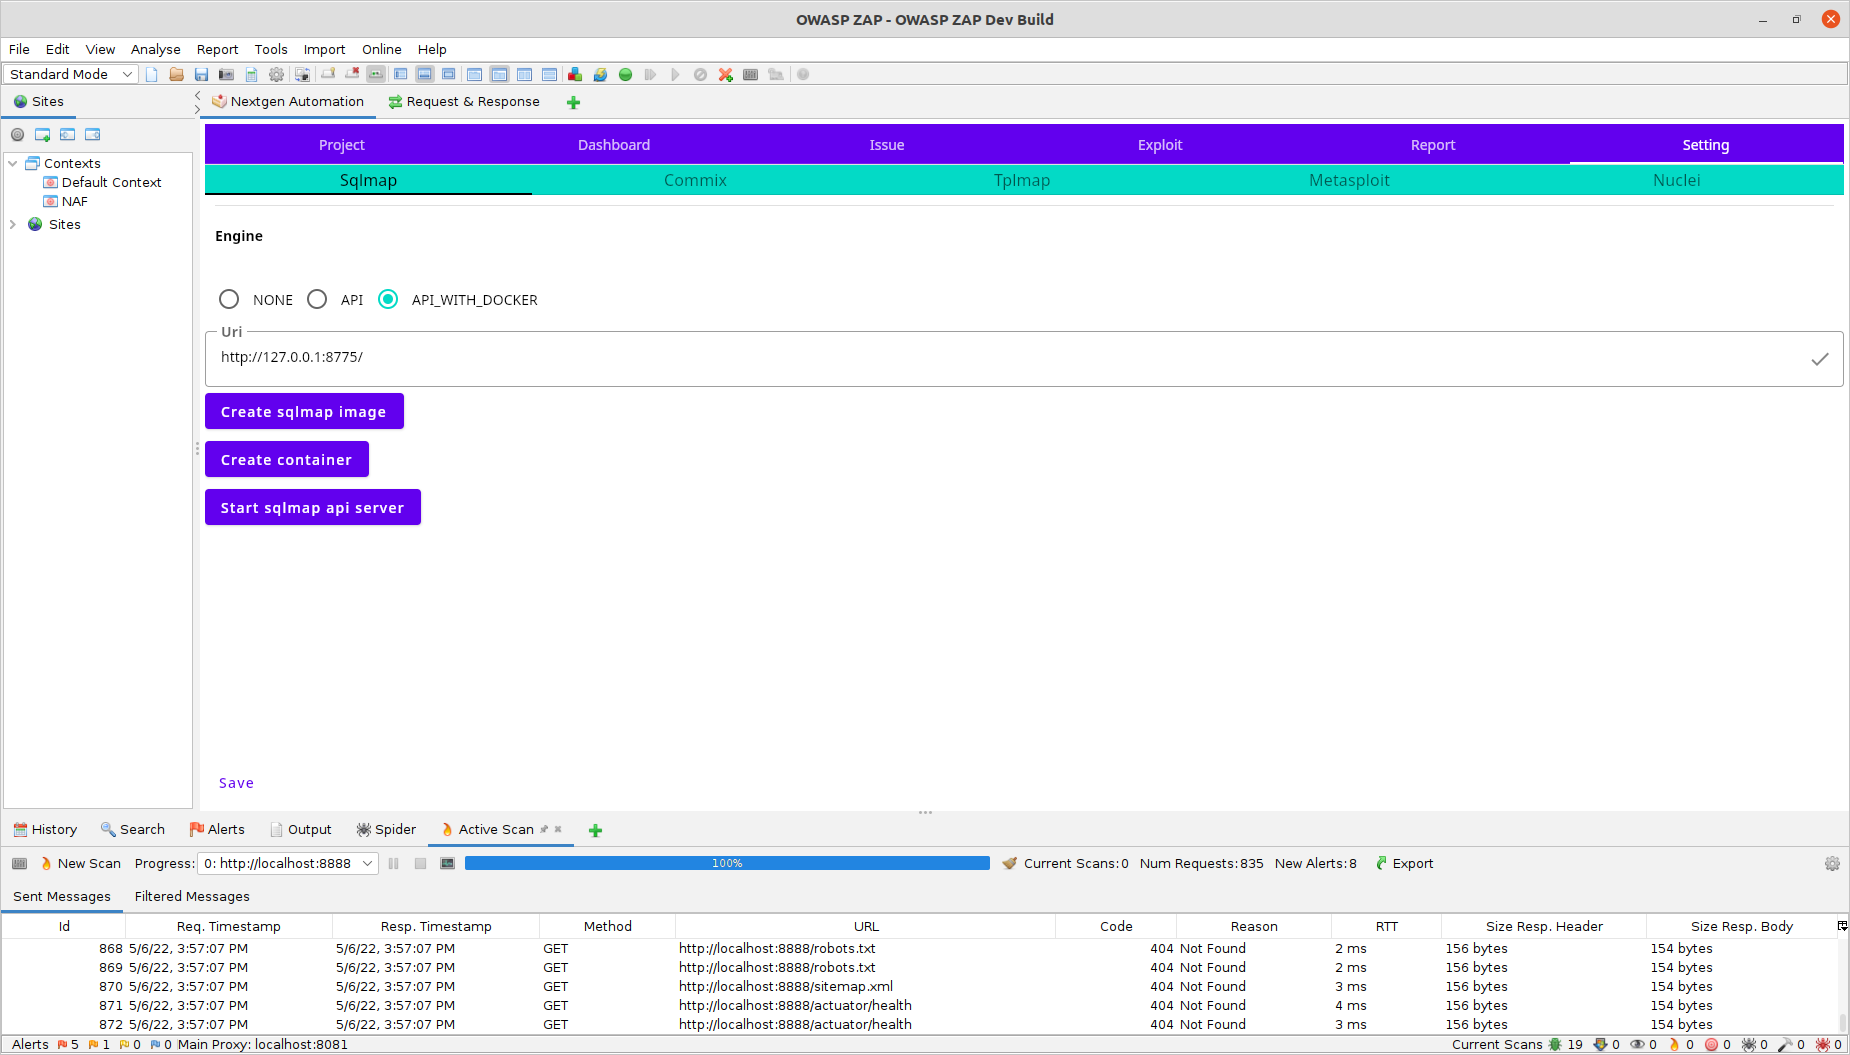
\includegraphics[width=\linewidth]{./images/docker.png}
	\caption{Quản lý Docker của từng thành phần}
	\label{fig:docker}
\end{figure}

\end{document}